% !TEX root = ../main.tex
%Este trabalho está licenciado sob a Licença Creative Commons Atribuição-CompartilhaIgual 3.0 Não Adaptada. Para ver uma cópia desta licença, visite https://creativecommons.org/licenses/by-sa/3.0/ ou envie uma carta para Creative Commons, PO Box 1866, Mountain View, CA 94042, USA.

\chapter{Curvas e trajetórias}\index{curvas e trajetórias}\index{trajetórias}
  Neste capítulo, estudamos funções vetoriais do tipo $\vec{r}(t)$, ou seja, uma função que associa um parâmetro real a vetores no plano ou espaço. Funções vetoriais que dependem de apenas uma variável são os exemplos mais simples de funções que estudaremos. 

\section{Funções vetoriais de uma variável - curvas e trajetórias}
Uma função vetorial de uma variável é uma função da forma $$\vec{r}:D\to \mathbb{R}^3,$$ onde $D\subseteq \mathbb{R}$ é o domínio de definição de $\vec{r}$ e $t$ é um parâmetro - podendo ser interpretado como o tempo ou não. Em coordenadas cartesianas, uma função vetorial assume a seguinte forma:
$$\vec{r}(t)=x(t)\vec{i}+y(t)\vec{j}+z(t)\vec{k}$$
onde $\vec{i}=(1;0;0)$,$\vec{j}=(0;1;0)$ e $\vec{k}=(0;0;1)$ são mostrados na figura \ref{fig_vetijk}.

\begin{figure} \label{fig_vetijk}
\begin{center}
    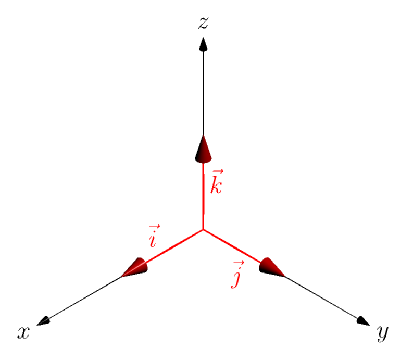
\includegraphics{./cap_curvas/figs/vetores_ijk}
 \caption{Os vetores canônicos $\vec{i},\vec{j},\vec{k}$.}
  \end{center}
\end{figure}

\begin{ex}\label{exfv01} São exemplos de funções vetoriais
\begin{itemize}
\item [a)] $\vec{f}(t)=\sin(t)\vec{i}+\cos(t)\vec{j}$
\item [b)] $\vec{g}(t)=t \vec{i}+\cosh(t)\vec{k}$
\item [c)] $\vec{h}(t)=2\cos(t)\vec{i}+4\sin(t)\vec{j}+t\vec{k},~~ 0\leq t \leq 8\pi$
\end{itemize}
\end{ex}  

Uma curva\index{curva} no espaço pode ser representada pelo conjunto de pontos de uma função vetorial $\vec{r}(t)$ não constante em todo o seu domínio. Um ponto $\vec{r}(t)$ de uma parametrização é dito regular se $\frac{d\vec{r}(t)}{dt} \neq 0$. Uma parametrização é dita regular\index{parametrização regular} em $t$ se $\frac{d\vec{r}(t)}{dt} \neq 0$ em todos os pontos. É possível definir orientação para uma curva regularmente parametrizada\index{orientação de uma curva}, a orientação é dada pelo sentido de crescimento do parâmetro $t$. 

\begin{ex}
A função vetorial $\vec{f}(t)=\cos(t)\vec{i}+\sin(t)\vec{j}$ para $0\leq t \leq 2\pi$ descreve  uma circunferência de raio 1 centrada na origem sobre o plano $xy$ orientada no sentido anti-horário.
\end{ex}

\begin{figure}%{0.35\textwidth}
\begin{center}
    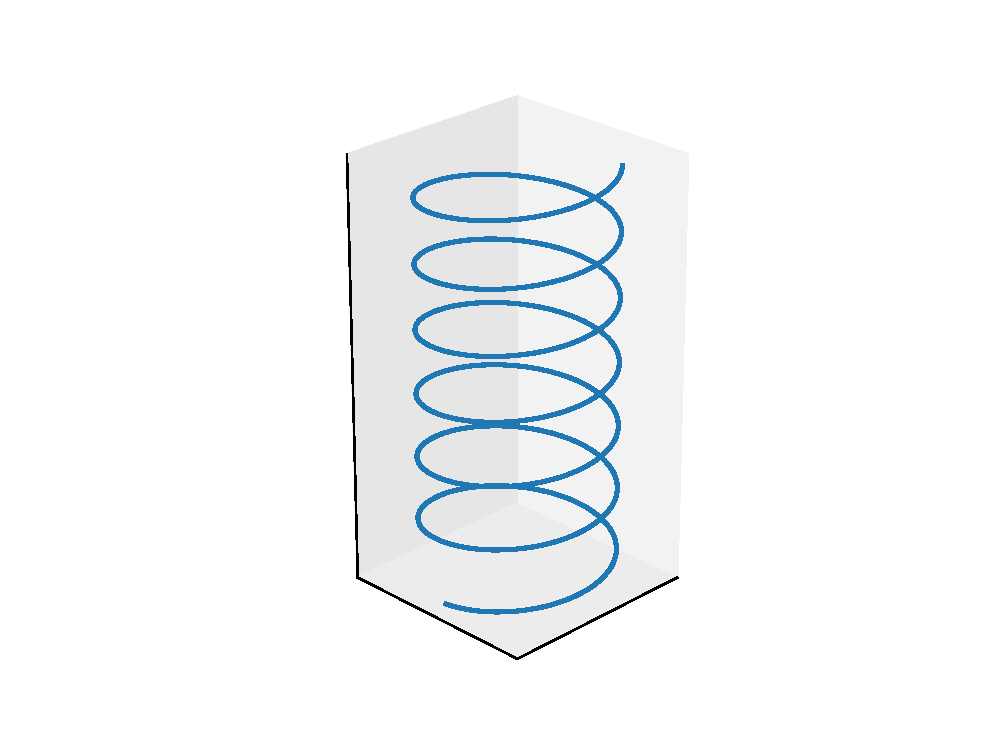
\includegraphics{./cap_curvas/figs/helice}
\caption{\label{helicedex}Hélice circular dextrogira associada à função vetorial do Exemplo~\ref{cap_curvas:exemplo_helice}.}
  \end{center}
\end{figure}

\begin{ex}\label{cap_curvas:exemplo_helice}
A função vetorial $\vec{f}(t)=\cos(t)\vec{i}+\sin(t)\vec{j}+t\vec{k}$ para $ t \in\mathbb{R}$ descreve uma hélice circular, como mostra a figura \ref{helicedex}.
\end{ex}

O limite\index{limite de uma função vetorial de uma variável}, a derivação\index{derivada de uma função vetorial de uma variável} e a integração vetorial\index{integral de uma função vetorial de uma variável} são definidas componente a componente no sistema de coordenadas cartesiano:
\begin{eqnarray}
\lim_{t\to a}\vec{r}(t)&=&\lim_{t\to a}x(t) \vec{i}+\lim_{t\to a}y(t)\vec{j}+\lim_{t\to a}z(t)\vec{k}\label{deflim}\\
\frac{d\vec{r}(t)}{dt}&=&\frac{d x(t)}{dt}\vec{i}+\frac{d y(t)}{dt}\vec{j}+\frac{d z(t)}{dt}\vec{k}\label{defder}\\
\int_{a}^b\vec{r}(t){dt}&=&\int_{a}^bx(t)dt~\!\vec{i}+\int_{a}^by(t)dt~\!\vec{j}+\int_{a}^bz(t)dt~\!\vec{k}\label{defint}\\
\int\vec{r}(t){dt}&=&\int x(t)dt~\!\vec{i}+\int y(t)dt~\!\vec{j}+\int z(t)dt~\!\vec{k}\label{defint2}
\end{eqnarray}

\begin{teo}[Regras de derivação] A derivada de funções vetoriais satisfaz as seguintes propriedades:
\begin{enumerate}
\item Se $\vec{r}(t)$ é um vetor constante, então $\frac{d\vec{r}(t)}{dt}=\vec{0}$. 
\item $\frac{d}{dt}\left[\alpha \vec{r}_1(t)+\beta \vec{r}_2(t)\right]=\alpha\frac{d\vec{r}_1(t)}{dt}+\beta\frac{d\vec{r}_2(t)}{dt}$
\item Se $f(t)$ é uma função real, então $\frac{d}{dt}\left[f(t) \vec{r}(t)\right]=f'(t)\vec{r}(t)+f(t)\frac{d\vec{r}(t)}{dt}$
\item $\frac{d}{dt}\left[\vec{r}_1(t)\cdot \vec{r}_2(t)\right]=\vec{r}_1(t)\cdot\frac{d\vec{r}_2(t)}{dt}+\frac{d\vec{r}_1(t)}{dt}\cdot\vec{r}_2(t)$
\item $\frac{d}{dt}\left[\vec{r}_1(t)\times \vec{r}_2(t)\right]=\vec{r}_1(t)\times\frac{d\vec{r}_2(t)}{dt}+\frac{d\vec{r}_1(t)}{dt}\times\vec{r}_2(t)$
\end{enumerate}
\end{teo}
\begin{proof} Os dois primeiros ítens podem ser obtidos diretamente de (\ref{defder}). A verificação fica a cargo do leitor. O item três pode ser obtido de  uma aplicação da regra da cadeia a (\ref{defder})\index{derivada do produto de um escalar por um vetor}:
\begin{eqnarray*}\frac{d}{dt}\left[f(t) \vec{r}(t)\right]&=& \frac{d}{dt}\left[f(t) {x}(t)\vec{i}+f(t) {y}(t)\vec{j}+f(t) {z}(t)\vec{k}\right]\\
&=&\left[f'(t) x(t)+f(t)x'(t)\right]\vec{i}+\left[f'(t) y(t)+f(t)y'(t)\right]\vec{j}+\left[f'(t) z(t)+f(t)z'(t)\right]\vec{k}\\
&=&f'(t)\left[x(t)\vec{i}+y(t)\vec{j}+z(t)\vec{k}\right]+f(t)\left[x'(t)\vec{i}+y'(t)\vec{j}+z'(t)\vec{k}\right]\\
&=&f'(t)\vec{r}(t)+f(t)\frac{d\vec{r}(t)}{dt}
\end{eqnarray*}

A derivada do produto escalar de duas funções vetoriais é dado por:\index{derivada do produto escalar}
\begin{eqnarray*}\frac{d}{dt}\left[\vec{r}_1(t)\cdot \vec{r}_2(t)\right]&=&\frac{d}{dt}\left[x_1(t)x_2(t)+y_1(t)y_2(t)+z_1(t)z_2(t)\right]\\
&=&
\left[x_1'(t)x_2(t)+x_1(t)x_2'(t)\right]+\left[y_1'(t)y_2(t)+y_1(t)y_2'(t)\right]
\\&+&\left[z_1'(t)z_2(t)+z_1(t)z_2'(t)\right]\\&=&\vec{r}_1(t)\cdot\frac{d\vec{r}_2(t)}{dt}+\frac{d\vec{r}_1(t)}{dt}\cdot\vec{r}_2(t)
\end{eqnarray*}
Finalmente a derivada do produto vetorial pode ser obtida de\index{derivada do produto vetorial}:
{\allowdisplaybreaks
\begin{eqnarray*}
\frac{d}{dt}\left[\vec{r}_1(t)\times \vec{r}_2(t)\right]&=&\frac{d}{dt}\left[y_1(t) z_2(t)-z_1(t)y_2(t)\right]\vec{i}\\
&+&\frac{d}{dt}\left[z_1(t) x_2(t)-x_1(t)z_2(t)\right]\vec{j}\\
&+&\frac{d}{dt}\left[x_1(t) y_2(t)-y_1(t)x_2(t)\right]\vec{k}\\
&=&\left[y_1'(t) z_2(t)+y_1(t) z_2'(t)-z_1'(t)y_2(t)-z_1(t)y_2'(t)\right]\vec{i}\\
&+&\left[z_1'(t) x_2(t)+z_1(t) x_2'(t)-x_1'(t)z_2(t)-x_1(t)z_2'(t)\right]\vec{j}\\
&+&\left[x_1'(t) y_2(t)+x_1(t) y_2'(t)-y_1'(t)x_2(t)-y_1(t)x_2'(t)\right]\vec{k}\\
&=&\left[y_1'(t) z_2(t)-z_1'(t)y_2(t)\right]\vec{i}\\
&+&\left[z_1'(t) x_2(t)-x_1'(t)z_2(t)\right]\vec{j}\\
&+&\left[x_1'(t) y_2(t)-y_1'(t)x_2(t)\right]\vec{k}\\
&+&\left[y_1(t) z_2'(t)-z_1(t)y_2'(t)\right]\vec{i}\\
&+&\left[z_1(t) x_2'(t)-x_1(t)z_2'(t)\right]\vec{j}\\
&+&\left[x_1(t) y_2'(t)-y_1(t)x_2'(t)\right]\vec{k}\\
&=&\vec{r}_1(t)\times\frac{d\vec{r}_2(t)}{dt}+\frac{d\vec{r}_1(t)}{dt}\times\vec{r}_2(t)
\end{eqnarray*}
}
\end{proof}

Demonstraremos agora um importante teorema do cálculo vetorial:
\begin{teo}\label{teodernormacst} Uma função vetorial $\vec{u}(t)$ possui norma constante se e somente se $\vec{u}(t)\cdot\frac{d\vec{u}(t)}{dt}=0$. 
\end{teo}
\begin{proof} Como $\|u\|^2=\vec{u}(t)\cdot\vec{u}(t)$, temos
$$\frac{d \|u\|^2}{dt}=\frac{d}{dt}\left[\vec{u}(t)\cdot\vec{u}(t)\right]=\vec{u}\cdot\frac{d\vec{u}}{dt}+\frac{d\vec{u}}{dt}\cdot\vec{u}=2\vec{u}\cdot\frac{d\vec{u}}{dt}$$
Assim, se $\|u\|$ for constante, a derivada à esquerda é nula e temos $\vec{u}(t)\cdot\frac{d\vec{u}(t)}{dt}=0$. Reciprocamente se $\vec{u}(t)\cdot\frac{d\vec{u}(t)}{dt}=0$, então $\|u\|$ deve ser constante.
\end{proof}
\begin{obs} Uma importante interpretação deste teorema é que se $\vec{v}(t)$ representa a velocidade de uma partícula no instante de tempo $t$, então se o módulo da velocidade, $v(t)$, for constante e não nulo então a aceleração $\vec{a}=\frac{d\vec{v}(t)}{dt}$ é perpendicular a $\vec{v}(t)$ sempre que for não nula.  
\end{obs}


%\subsection*{Exercícios resolvidos}





\subsection*{Exercícios}

\begin{exer}Calcule as derivadas das funções vetoriais do exemplo \ref{exfv01}:
\begin{itemize}
\item [a)] $\vec{f}(t)=\sin(t)\vec{i}+\cos(t)\vec{j}$
\item [b)] $\vec{g}(t)=t \vec{i}+\cosh(t)\vec{k}$
\item [c)] $\vec{h}(t)=2\cos(t)\vec{i}+4\sin(t)\vec{j}+t\vec{k},~~ 0\leq t \leq 8\pi$
\end{itemize}
\end{exer}

\begin{resp} $\vec{f'}(t)=\cos(t)\vec{i}-\sin(t)\vec{j}$,~~ $\vec{g'}(t)= \vec{i}+\sinh(t)\vec{k}$, ~~$\vec{h'}(t)=\cos(t)\vec{i}-\sin(t)\vec{j}+\vec{k}$\end{resp}
\begin{exer} Dada a função vetorial $\vec{r}(t)=t^2\vec{i}+e^t\vec{j}-2\cos\pi t ~\! \vec{k}$, calcule:
\begin{itemize}
\item [a)] $\displaystyle \lim_{t\to 0} \vec{r}(t)$
\item [b)] $\displaystyle \frac{d \vec{r}(t)}{dt}$
\item [c)] $\displaystyle \frac{d\vec{r}(1)}{dt}$
\item [d)] $\displaystyle \int_0^1 \vec{r}(t)dt$
\item [e)] $\displaystyle \int \vec{r}(t)dt$
\end{itemize}
\end{exer}
\begin{resp} $\vec{j}-2\vec{k}$, $\frac{\vec{r(t)}}{dt}=2t\vec{i}+e^t\vec{j}+2\pi\sin\pi t ~\! \vec{k}$, $\frac{\vec{r}(1)}{dt}=2\vec{i}+e\vec{j}$, $\frac{1}{3}\vec{i}+(e-1)\vec{j}$, $\left(\frac{1}{3}t^3+C_1\right)\vec{i}+\left(e^t+C_2\right)\vec{j}+\left(-\frac{2}{\pi}\sin\pi t+C_3\right)\vec{k}$
\end{resp}
\begin{exer}Encontre o domínio da função vetorial $\vec{r}(t)$ e o valor da função no ponto $t_0$ para:
\begin{itemize}
 \item[a)] $\vec{r}=\cos(t)\vec{i}-3t\vec{j}$; $t_0=\pi$.
 \item[b)] $\vec{r}=\cos(\pi t)\vec{i}-\ln(t)\vec{j}+\sqrt{t-2}$; $t_0=3$.
\end{itemize}
\end{exer}
\begin{exer}Expresse as equações paramétricas abaixo como uma única equação vetorial:
\begin{itemize}
 \item[a)] $x(t)=2\cos(t)$; $y(t)=t+\sin(t)$.
 \item[b)] $x(t)=2t$; $y(t)=2\sin(3t)$; $z(t)=5\cos(3t)$.
\end{itemize}
\end{exer}
\begin{exer}Encontre a declividade (coeficiente angular) da reta contida no plano $z=0$ representada por $\vec{r}=(1-2t)\vec{i}+(2-3t)\vec{j}$
\end{exer}
\begin{resp}
 -$\frac{3}{2}$
\end{resp}
\begin{exer} Reconheça e represente graficamente as curvas descritas pelas seguintes funções vetoriais:
\begin{itemize}
\item [a)] $\vec{f}(t)=\sin(t)\vec{i}+\cos(t)\vec{j}+\vec{k}$, $0\leq t \leq \pi$
\item [b)] $\vec{f}(t)=\sin(t)\vec{i}+2\cos(t)\vec{k}$, $0\leq t \leq 2\pi$
\item [c)] $\vec{f}(t)=\sin(t)\vec{i}+\cos(t)\vec{k}$, $-\infty < t < \infty$
\item [d)] $\vec{f}(t)=t\vec{i}+\sqrt{4-t^2}~\!\vec{j}$, $-2 \leq t \leq 2$
\item [e)] $\vec{f}(t)=t\vec{i}+\cosh(t)\vec{j}$, $-\infty < t < \infty $
\item [f)] $\vec{f}(t)=\sinh(t)\vec{i}+\cosh(t)\vec{j}$, $-\infty < t< \infty $
\end{itemize} 
\end{exer}
\begin{resp} Semicircunferência de raio 1 centrada em $(0,0,1)$ sobre o plano $z=1$. Elipse de semi-eixos $1$ e $2$ centrada na origem sobre o plano $xz$. Hélice circular levogira de raio $1$ e passo $2\pi$.  Semicircunferência de raio 2 centrada na origem sobre o plano $xy$ e $y\geq 0$. Uma catenária sobre o plano $xy$. Uma hipérbole. 
\end{resp}
\begin{exer}Dada a hélice circular $\vec{r}(t)=a\cos(t)\vec{i}+a\sin(t)\vec{j}+ct\vec{k}$, sendo $c>0$, encontre $c$ tal que a cada volta completa $z$ avance $3$ unidades.
 \end{exer}
\begin{exer}Seja $\vec{r}(t)$ o vetor posição de uma partícula dado por
$$\vec{r}(t)=a\cos(wt)\vec{i}+a\sin(wt)\vec{j}$$
Calcule o vetor velocidade $\vec{v}$ e o vetor aceleração $\vec{a}$ dados por $\vec{v}=\frac{d\vec{r}(t)}{dt}$ e $\vec{a}=\frac{d\vec{v}(t)}{dt}$.
\end{exer}



\begin{exer} Verifique que a função vetorial dada por $\vec{f}(t)=\frac{1-t^2}{1+t^2}\vec{i}+\frac{2t}{1+t^2}\vec{j}$, $-\infty<t<\infty$
representa uma curva contida em uma circunferência no plano $xy$  centrada na origem. Identifique o raio desta circunferência, identifique a curva e isole os quatro quadrantes.
\end{exer}

\begin{resp}raio=$1$, centro na origem. $Q1: 0<t<1$, $Q2:t>1$, $Q3:t<-1$, $Q4:-1<t<0$. A curva é a circunferência menos o ponto $\left<-1,0\right>$.
\end{resp}

\begin{exer}
Sendo $\hat{r}(t)=\frac{1}{r(t)} \vec{r}(t)$, onde $r(t)=\|\vec{r}(t)\|$,  mostre as seguintes identidades:
\begin{itemize}
\item[a)] $\displaystyle r'(t) = \frac{d\vec{r}(t)}{dt}\cdot \hat{r}(t)$
\item[b)] $\displaystyle \frac{d}{dt}\left[\vec{r}(t)\times\frac{d\vec{r}(t)}{dt}\right]=\vec{r}(t)\times\frac{d^2\vec{r}(t)}{dt^2}$ 
\item[c)] $\displaystyle r'(t)=\frac{\vec{r}(t)\cdot\frac{d\vec{r}(t)}{dt}}{r(t)}$ 
\item[d)] $\displaystyle \frac{d\hat{r}(t)}{dt}=\frac{1}{r(t)} \frac{d\vec{r}(t)}{dt}-\frac{\vec{r}(t)\cdot\frac{d\vec{r}(t)}{dt}}{r(t)^3} \vec{r}(t)$
\end{itemize}
\end{exer}
\begin{resp}
a) $\|\hat{r}\|$ constante implica $\hat{r} \cdot \frac{d\hat{r}}{dt}=0$. Ademais, $ \frac{d\vec{r}}{dt} = \frac{d(r \hat{r})}{dt} = r' \hat{r} + r \frac{d\hat{r}}{dt} \Rightarrow \frac{d\vec{r}}{dt} \cdot \hat{r} = 
r' \|\hat{r}\|^2 + r \frac{d\hat{r}}{dt} \cdot \hat{r} = r' $ 
. b) $\frac{d}{dt} \left[ \vec{r} \times \frac{d\vec{r}}{dt} \right] =
\frac{d \vec{r}}{dt} \times \frac{d \vec{r}}{dt} + \vec{r} \times \frac{d^2 \vec{r}}{dt^2} = \vec{r} \times \frac{d^2 \vec{r}}{dt^2} $. c) a partir de a), multiplica numerador e denominador por $r(t)$. d) $\frac{d\hat{r}}{dt} = 
\frac{d}{dt} \left( r^{-1} \vec{r} \right) = \frac{d}{dt} \left( r^{-1} \right) \vec{r} + r^{-1} \frac{d \vec{r}}{dt} = \frac{1}{r} \frac{d\vec{r}}{dt} - \frac{r'}{r^2} \vec{r} = \frac{1}{r} \frac{d \vec{r}}{dt} - \frac{ \vec{r} \cdot \frac{d \vec{r}}{dt} }{r^3} \vec{r} $ pela parte c). 
\end{resp}
\begin{exer}Dadas $\vec{u}(t)=t^2\vec{i}-3t\vec{k}$, $\vec{v}(t)=-4t^3\vec{j}+(t+1)\vec{k}$ e $\vec{w}(t)=3t^2\vec{i}+t\vec{j}-t^3\vec{k}$, encontre:
\begin{itemize}
 \item[a)] $(\vec{u}\cdot \vec{v})'$.
 \item[b)] $(\vec{u}\times \vec{v})'$.
 \item[c)] $\left[\vec{u}\times (\vec{v}+\vec{w})\right]'$.
\end{itemize}
\end{exer}
\begin{resp}
\begin{itemize}
 \item[a)] $-3(2t+1)$.
 \item[b)] $-48t^3\vec{i}-(3t^2+2t)\vec{j}-20t^4\vec{k}$.
 \item[c)] $(6t-48t^3)\vec{i}-(2t+30t^2-5t^4)\vec{j}+(3t^2-20t^4)\vec{k}$.
\end{itemize} 
\end{resp}
\section{Comprimento de arco}
Dada uma curva parametrizada pela função vetorial $\vec{r}(t)=x(t)\vec{i}+y(t)\vec{j}+z(t)\vec{k}$, $t\in[a,b]$, estamos interessados no problema de calcular o comprimento $L$ do arco de descrito por uma curva $\vec{r}(t)$, $a\leq t\leq b$.
  
\begin{figure}
\centering
    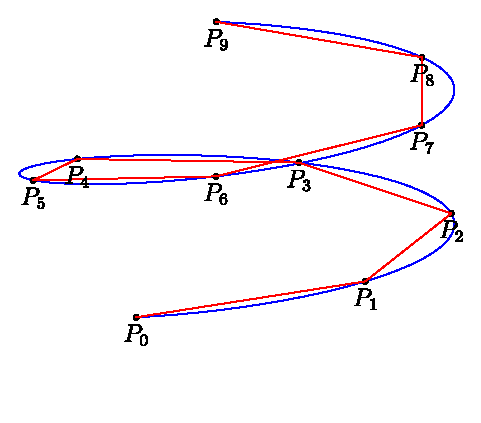
\includegraphics{./cap_curvas/figs/helice_retificacao}
\caption{Aproximação poligonal do comprimento do arco}\label{fig_compr_arc}
\end{figure}

 
 
Seja $a=t_0<t_1<t_2<\cdots<t_n=b $ uma partição equidistante do domínio com $\Delta t=t_i-t_{i-1}$ e $P_i=\vec{r}(t_i)$, $i=0,1,\cdots,n$, pontos sobre a curva, como mostra a figura \ref{fig_compr_arc}. Uma possível aproximação para o comprimento da curva é dado pelo comprimento da poligonal determinada por essa partição. Observe que o comprimento do segmento $P_{i-1}P_i$ é dado por $\|P_i-P_{i-1}\|$, logo, a aproximação para o comprimento da curva é
\begin{eqnarray*}
L_n&=&\sum_{i=1}^n\|P_i-P_{i-1}\|\\
&=&\sum_{i=1}^n \sqrt{(x_i-x_{i-1})^2+(y_i-y_{i-1})^2+(z_i-z_{i-1})^2}\\
&=&\sum_{i=1}^n \Delta t \sqrt{\frac{(x_i-x_{i-1})^2}{(\Delta t) ^2}+\frac{(y_i-y_{i-1})^2}{(\Delta t) ^2}+\frac{(z_i-z_{i-1})^2}{(\Delta t) ^2}}\\
&=&\sum_{i=1}^n \sqrt{\left(\frac{x_i-x_{i-1}}{\Delta t }\right)^2+\left(\frac{y_i-y_{i-1}}{\Delta t}\right)^2+\left(\frac{z_i-z_{i-1}}{\Delta t}\right)^2}\Delta t.
\end{eqnarray*}
Naturalmente, $L=\lim_{n\to\infty }L_n$. Como o lado direito da última igualdade é uma soma de Riemann, temos:
\begin{equation}\label{defcomparco}
L=\int_{a}^{b} \sqrt{\left(\frac{dx(t)}{dt}\right)^2+\left(\frac{dy(t)}{dt}\right)^2+\left(\frac{dz(t)}{dt}\right)^2}dt=\int_{a}^{b}\left\|\frac{d\vec{r}(t)}{dt}\right\|dt.
\end{equation}
Logo, o comprimento do arco $s$ quando a parâmetro corre de $a$ até $t$ é
\begin{equation}\label{defcomparco_1}
s(t)=\int_{a}^{t}\left\|\frac{d\vec{r}(\tau)}{dt}\right\|d\tau,\qquad a\leq t\leq b.
\end{equation}

\subsection*{Exercícios resolvidos}

\begin{exer} \label{exe_co_arc1}
Mostre que o comprimento de arco da curva parametrizada $\vec{r}(t) = t \vec{i} + t^2 \vec{j}$, definida para $-2 \leq t \leq 2$ é $L = 2\sqrt{17} + \frac{\ln(4+\sqrt{17})}{2}$. Tal curva pertence à parábola $y=x^2$, e pode ser visualizada na figura \ref{fig_co_arc1}.
\end{exer}

\begin{figure}
\centering
    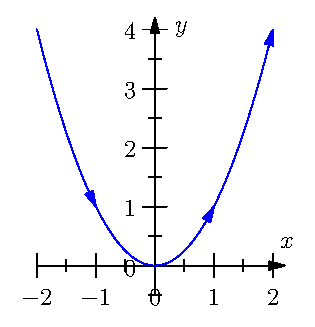
\includegraphics{./cap_curvas/figs/comprimento_arco_parabola}
    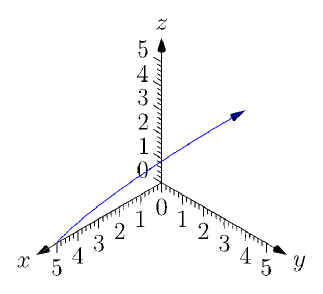
\includegraphics{./cap_curvas/figs/comprimento_arco_curva}
\caption{(esq) Curva do exercício E \ref{exe_co_arc1}; (dir) curva do exercício E \ref{exe_co_arc2}.}\label{fig_co_arc1}
\end{figure}

$\frac{d\vec{r}}{dt} = \vec{i} + 2t \vec{j} $ e portanto $L = \int_{-2}^2 \sqrt{4t^2 + 1} dt = 2 \int_0^2 \sqrt{4t^2+1}dt$. Com a mudança de variável $2t = \tan(u), 0 \leq u \leq \alpha$, onde $\alpha=\arctan(4)$ temos $2dt = \sec^2(u)du$ e então $L =  \int_0^{\alpha} |\sec(u)| \sec^2(u) du = \int_0^{\alpha} \sec^3(u)du = \left[ \frac{\sec(u)\tan(u) + \ln|\sec(u)+\tan(u)|}{2} \right]_0^{\arctan(4)} $.

\begin{exer} \label{exe_co_arc2}
Mostre que o comprimento de arco da curva parametrizada $\vec{r}(t) = 5(1-t^2) \vec{i} + 4 t^{5/2}\vec{j} + 5t^2 \vec{k}$, definida para $0 \leq t \leq 1$ é $ L = \frac{32}{3} \sqrt{2} - 4\sqrt{3}$. Essa curva pode ser visualizada na figura \ref{fig_co_arc1}. 
\end{exer}


$\frac{d\vec{r}}{dt} = -10t \vec{i} + 10 t^{3/2} \vec{j} + 10t \vec{k} $ e portanto $L = \int_0^1 \sqrt{ 100 t^3 + 100 t^2 + 100t^2 } dt = 10 \int_0^1 t \sqrt{t+2} dt = 10 \int_2^3 (s-2) s^{1/2} ds = 10 \int_2^3 (s^{3/2}-2s^{1/2})ds$



\subsection*{Exercícios}

\begin{exer} \label{exe_co_arc3}
Mostre que o comprimento de arco da curva parametrizada $\vec{r}(t) = (1+t) \vec{i} + (1-t^2)\vec{j}$, definida para $-1 \leq t \leq 1$ é $ L = \sqrt{5} + \frac{\ln(\sqrt{5}+2)}{2}$.
\end{exer}


\begin{exer} \label{exe_co_arc4}
Mostre que o comprimento de arco da curva parametrizada $\vec{r}(t) = (1-t^2) \vec{i} + (t^2+t^3) \vec{j} + (1+t^2-t^3)\vec{k}$, definida para $0 \leq t \leq 1$ é $ L = \frac{5 \sqrt{30}-4\sqrt{3}}{9} $.
\end{exer}

\begin{exer} \label{exe_co_arc5}
Mostre que o comprimento de arco da curva parametrizada $\vec{r}(t) = 2t^3 \vec{i} + (1-t^3+2t^{9/2}) \vec{j} + (t^3+2t^{9/2})\vec{k}$, definida para $0 \leq t \leq 1$ é $ L = \frac{14\sqrt{6}}{9} $.
\end{exer}



\section{Triedro de Frenet-Serret}

Seja a curva descrita pela função vetorial $\vec{r}(t)$. Queremos encontrar um vetor que seja tangente à curva em um dado ponto\index{vetor tangente}. Para tal tomamos o limite
$$\lim_{h\to 0} \frac{\vec{r}(t+h)-\vec{r}(t)}{h}$$  
Este limite converge para $\frac{d\vec{r}(t)}{dt}$ e, geometricamente, para o vetor tangente à curva no ponto $P$ relativo a $\vec{r}(t)$\footnote{O leitor atento ao formalismo pode tomar esta como uma definição de vetor tangente. Adiante, veremos que esta definição é consistente com o vetor tangente do cálculo de funções de uma variável.} sempre que $\frac{d\vec{r}(t)}{dt} \neq \vec{0}$. O sentido do vetor $\frac{d\vec{r}(t)}{dt}$ é dado pela parametrização da curva, em outras palavras, o vetor $\frac{d\vec{r}(t)}{dt}$ aponta no sentido em que o parâmetro $t$ cresce.


\begin{figure}%{0.35\textwidth}
\begin{center}
    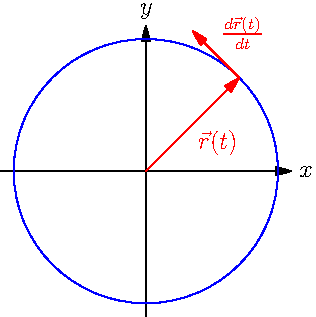
\includegraphics{./cap_curvas/figs/vetor_tangente_circunferencia}
\caption{O vetor tangente $\frac{d\vec{r}(t)}{dt}$}\label{circtang}
  \end{center}
\end{figure}


Observe que a norma do vetor tangente depende de como a curva é parametrizada e não apenas da curva em si. A fim de trabalhar com um objeto que independe da parametrização, é natural definirmos o vetor tangente unitário\index{vetor tangente unitário}, denotado por $\vec{T}$ (veja figura \ref{Frenet_Serret}):
\begin{equation}\label{defvecunit}
\vec{T}(t)=\frac{1}{\left\|\frac{d\vec{r}(t)}{dt}\right\|}\frac{d\vec{r}(t)}{dt},\qquad \frac{d\vec{r}(t)}{dt} \neq \vec{0}.
\end{equation} 
A condição de existência para o vetor $\vec{T}$ é que a função vetorial que parametriza a curva seja diferenciável e que sua derivada seja diferente de zero, ou seja, que a parametrização seja regular.

\begin{obs} Quando $\vec{r}(t)$ representa a trajetória de uma partícula ao longo do tempo, a derivada $\frac{d\vec{r}(t)}{dt} $ é a velocidade $\vec{v}(t)$ da partícula. Neste caso, o vetor tangente unitário é o versor associado a $\vec{v}(t)$:
$$\vec{v}(t)=v(t) \hat{v}(t)=v(t) \vec{T}(t).$$
A norma de $\vec{v}(t)$, denotada por $v(t)$, é chamada de velocidade escalar\index{velocidade escalar}. O vetor $\vec{T}(t)$ indica o sentido e a direção da velocidade.
\end{obs}

O vetor $\vec{T}$ pode ser definido de forma alternativa como segue: consideramos $s$ como função de $t$ na expressão (\ref{defcomparco_1}) e observamos que $s'(t)=\left\|\frac{d\vec{r}(t)}{dt}\right\|>0$. Assim, $s(t)$ é uma função contínua e monótona de $t$. Por outro lado, usando a Regra da Cadeia, temos:
$$
\frac{d\vec{r}}{dt}=\frac{d\vec{r}}{ds}\frac{ds}{dt}=\frac{d\vec{r}}{ds}\left\|\frac{d\vec{r}(t)}{dt}\right\|.
$$
Como $\frac{d\vec{r}(t)}{dt}$ representa o vetor tangente, então
$$
\frac{d\vec{r}}{ds}=\frac{1}{\|\frac{d\vec{r}(t)}{dt}\|}\frac{d\vec{r}}{dt}=\vec{T}
$$
representa um vetor tangente unitário.


\begin{figure}%{0.35\textwidth}
\begin{center}
    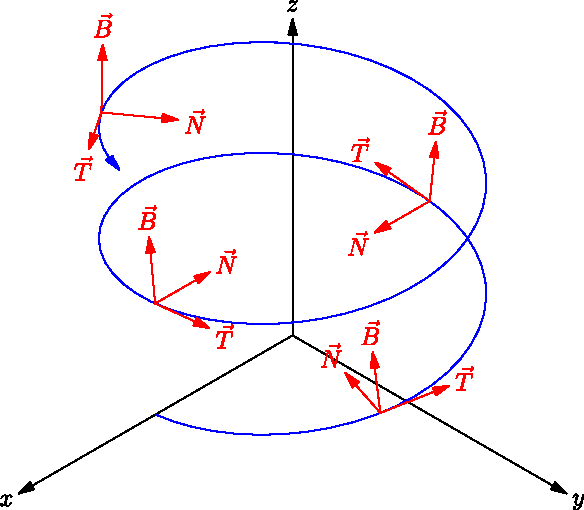
\includegraphics{./cap_curvas/figs/helice_TNB}
\caption{Triedro de Frenet-Serret}\label{Frenet_Serret}
  \end{center}
\end{figure}


Agora, queremos definir um vetor ortogonal a $\vec{T}$ que esteja no plano determinado por $\frac{d\vec{r}(t)}{dt}$ e $\frac{d^2\vec{r}(t)}{dt^2}$. Para isso, usamos o resultado do teorema \ref{teodernormacst}. Observe que a função vetorial $\vec{T}(t)$ possui módulo constante e, portanto, $\vec{T}(t)\cdot \frac{d\vec{T}(t)}{dt}=0$. Observe ainda que 
$$
\frac{d^2\vec{r}(t)}{dt^2}=\frac{d (v \vec{T} )}{dt} = v'(t) \vec{T}(t) + v(t) \frac{d \vec{T}(t)}{dt} = \frac{v'(t)}{v(t)} \frac{d\vec{r}(t)}{dt}+ v(t) \frac{d\vec{T}(t)}{dt}
$$
implica
$$ \frac{d\vec{T}(t)}{dt} = \frac{1}{v(t)} \frac{d^2 \vec{r}(t)}{dt^2} - \frac{v'(t)}{v(t)^2} \frac{d \vec{r}(t)}{dt}
$$
e assim 
$\vec{T}(t)$ e $\frac{d\vec{T}(t)}{dt}$ pertencem ao plano gerado por $\frac{d\vec{r}(t)}{dt} $ e $\frac{d^2\vec{r}(t)}{dt^2}$ e são ortogonais entre si. Entretanto, $\frac{d\vec{T}(t)}{dt}$ não é necessariamente unitário. Logo, faz sentido definir o vetor normal unitário\index{vetor normal unitário} como
$$
\vec{N}=\frac{1}{\left\|\frac{d\vec{T}(t)}{dt}\right\|} \frac{d \vec{T}(t)}{dt}.
$$
A figura \ref{Frenet_Serret} contém a representação do triedro de Frenet-Serret em alguns pontos de uma hélice dextrogira.

Finalmente, vamos definir um vetor unitário que é simultanemente ortogonal a $\vec{T}$ e $\vec{N}$. A forma natural de obter um vetor ortogonal a outros dois vem do produto vetorial. Assim, o vetor binormal unitário\index{vetor binormal unitário} é definido como
$$
\vec{B}=\vec{T}\times\vec{N}.
$$
Das propriedades de produto vetorial, temos que $\vec{B}$, além de ortogonal a $\vec{T}$ e $\vec{N}$, é unitário e forma um sistema dextrogiro. O trio $\vec{T}$, $\vec{N}$ e $\vec{B}$ é chamado de triedro de Frenet-Serret. A figura \ref{Frenet_Serret} apresenta a representação de alguns triedros de Frenet-Serret.


\subsection*{Exercícios resolvidos}




\begin{exeresol}
  Considere a curva $\vec{r}(t)$ definida no exercício E \ref{exe_co_arc4}. Encontre o triedro de Frenet-Serret $\vec{T}$, $\vec{N}$ e $\vec{B}$.
\end{exeresol}
\begin{resol}
 $\vec{v}(t) = \frac{d \vec{r}}{dt} = -2t \vec{i} + t(2+3t) \vec{j} + t(2-3t)\vec{k}$. Então $\left\|\vec{v} \right\|^2 = 4t^2 + t^2(2+3t)^2 + t^2(2-3t)^2 = t^2(12+18t^2)$ e assim $\vec{T} = \frac{\vec{v}}{\|\vec{v}\|} = \frac{-2 }{\sqrt{12+18t^2}}\vec{i} + \frac{2+3t}{\sqrt{12+18t^2}}\vec{j} + \frac{2-3t}{\sqrt{12+18t^2}}\vec{k}$. Derivando em relação a $t$: $\frac{d\vec{T}}{dt} = \frac{36t}{(12+18t^2)^{3/2}} \vec{i} + \frac{36(1-t)}{(12+18t^2)^{3/2}} \vec{j} - \frac{36(1+t)}{(12+18t^2)^{3/2}} \vec{k} $ e para normalizar sem trocar seu sentido definimos $\vec{u} = t \vec{i} + (1-t) \vec{j} - (1+t)\vec{k}$, que implica $\|\vec{u}\|^2=t^2 + (1-t)^2 + (1+t)^2 = 3t^2 + 2$, e então $\vec{N} = \frac{\frac{d\vec{v}}{dt}}{\|\frac{d\vec{v}}{dt}\|} = \frac{\vec{u}}{\|\vec{u}\|}=\frac{t}{\sqrt{3t^2+2}} \vec{i} + \frac{1-t}{\sqrt{3t^2+2}} \vec{j} - \frac{1+t}{\sqrt{3t^2+2}} \vec{k}$. Finalmente $ \vec{B} = \vec{T} \times \vec{N}$ calculado via $\left| \begin{array}{ccc}
\vec{i} & \vec{j} & \vec{k} \\
\frac{-2}{\sqrt{12+18t^2}} & \frac{2+3t}{\sqrt{12+18t^2}} & \frac{2-3t}{\sqrt{12+18t^2}} \\
\frac{t}{\sqrt{3t^2+2}} & \frac{1-t}{\sqrt{3t^2+2}} &  \frac{-1-t}{\sqrt{3t^2+2}} \end{array} \right| = \frac{(-4-6t^2)\vec{i} - (2+3t^2)\vec{j} - (2+3t^2)\vec{k}}{ \sqrt{12+18t^2} \sqrt{3t^2+2}} = \frac{-2}{\sqrt{6}} \vec{i} - \frac{1}{\sqrt{6}} \vec{j} - \frac{1}{\sqrt{6}} \vec{k}$.
\end{resol}

\begin{exeresol}
Um erro comum entre estudantes é substituir a definição de vetor binormal unitário $\vec{B}=\vec{T}\times\vec{N}$ pela expressão espúria dada por $$\frac{\frac{d\vec{N}}{dt}}{\left\|\frac{d\vec{N}}{dt}\right\|}.$$ Calcule esta expressão para o movimento circular uniforme e verifique que ela é igual a $-\vec{T}$ e, portanto, perpendicular a $\vec{B}$.
\end{exeresol}
\begin{resol}
 Considere $a$ e $w$ constantes positivas e a trajetória dada por:
 \begin{eqnarray*}
\vec{r}(t)&=&a\cos(wt)\vec{i}+a\sin(wt)\vec{j}\\
\vec{r}~\!'(t)&=&-aw\sin(wt)\vec{i}+aw\cos(wt)\vec{j}\\
\|\vec{r}~\!'(t)\|&=&|aw|=aw.
 \end{eqnarray*}

 \begin{eqnarray*}
\vec{T}(t)&=&\frac{\vec{r}~\!'(t)}{\|\vec{r}~\!'(t)\|}\\
 &=&\frac{-aw\sin(wt)\vec{i}+aw\cos(wt)\vec{j}}{aw}\\
 &=&{-\sin(wt)\vec{i}+\cos(wt)\vec{j}}\\
 \end{eqnarray*}
 
 \begin{eqnarray*}
\vec{N}(t)&=&\frac{\vec{T}~\!'(t)}{\|\vec{T}~\!'(t)\|}\\
  &=&\frac{-w\cos(wt)-w\sin(wt)}{w}\\
  &=&{-\cos(wt)-\sin(wt)}
 \end{eqnarray*}
 
 \begin{eqnarray*}
\frac{\vec{N}~\!'(t)}{\|\vec{N}~\!'(t)\|}\\
  &=&\frac{w\sin(wt)-w\cos(wt)}{w}\\
  &=&{\sin(wt)-\cos(wt)}=-\vec{T}
 \end{eqnarray*}
\end{resol}

\subsection*{Exercícios}
\begin{exer}Calcule $\vec{r}'(t_0)$ e esboce o gráfico de $\vec{r}(t)$ juntamente com o vetor tangente $\vec{r}'(t_0)$.
\begin{itemize}
 \item[a)] $\vec{r}(t)=t\vec{i}+t^2\vec{j}$, $t_0=2$.
 \item[b)] $\vec{r}(t)=e^{-t}\vec{i}+e^{2t}\vec{j}$, $t_0=\ln(2)$.
 \item[c)] $\vec{r}(t)=2\sin(t)\vec{i}+\vec{j}+2\cos(t)\vec{k}$, $t_0=\frac{\pi}{2}$.
 \end{itemize}
\end{exer}
\begin{exer}
Encontre os vetores unitários $\vec{T}$ e $\vec{N}$ para as curvas abaixo em $t=t_0$.
\begin{itemize}
 \item[a)] $\vec{r}(t)=5\cos(t)\vec{i}+5\sin(t)\vec{j}$, $t_0=\frac{\pi}{3}$.
 \item[b)] $\vec{r}(t)=(t^2-1)\vec{i}+t\vec{j}$, $t_0=1$.
\end{itemize}
\end{exer}
\begin{resp}
 \begin{itemize}
  \item[a)]$\vec{T}=\left(-\frac{\sqrt{3}}{2},\frac{1}{2}\right)$, $\vec{N}=\left(-\frac{1}{2},-\frac{\sqrt{3}}{2}\right)$.
  \item[a)]$\vec{T}=\left(\frac{2}{\sqrt{5}},\frac{1}{\sqrt{5}}\right)$, $\vec{N}=\left(\frac{1}{\sqrt{5}},-\frac{2}{\sqrt{5}}\right)$.
 \end{itemize}

\end{resp}

\begin{exer} Represente graficamente o terno de vetores $\vec{T}$,$\vec{N}$ e $\vec{B}$ e verifique através da regra da mão direita as seguintes identidades:
\begin{itemize}
\item[a)]$\vec{B}=\vec{T}\times\vec{N}$
\item[b)]$\vec{T}=\vec{N}\times\vec{B}$
\item[c)]$\vec{N}=\vec{B}\times\vec{T}$
\end{itemize}
Use a identidade vetorial dada por
$$\vec{u}\times\left(\vec{v}\times\vec{w}\right)=\vec{v}\left(\vec{u}\cdot\vec{w}\right)-\vec{w}\left(\vec{u}\cdot\vec{v}\right)$$ para obter as identidades $b$ e $c$ a partir de $a$.
\end{exer}
\begin{exer}\label{exer_formula_binormal}
 O vetor binormal unitário foi definido em aula como $\vec{B}(t)=\vec{T}(t)\times\vec{N}(t)$. Argumente, sem cálculos, que ele também poderia ser definido como 
 $$
 \vec{B}(t)=\frac{\vec{r}'(t)\times \vec{r}''(t)}{\|\vec{r}'(t)\times \vec{r}''(t)\|}.
 $$
\end{exer}
\begin{exer}
 Use a fórmula do exercício \ref{exer_formula_binormal} para calcular $\vec{B}(t)$ para a curva $C:$ $\vec{r}(t)=(\sin(t)-t\cos(t))\vec{i}+(\cos(t)+t\sin(t))\vec{j}+\vec{k}$.
\end{exer}
\begin{resp}
 $\vec{B}(t)=-\vec{k}$.
\end{resp}




\begin{exer} Considere a trajetória dada pela equações paramétricas
\begin{eqnarray*}
x&=&t\sin (t)\\
y&=&t\cos (t)\\
z&=&0
\end{eqnarray*}
Esboce gráfico dessa trajetória para $0\leq t \leq 2\pi$, indicando os pontos inicial e final. Esboce o triedro $\vec{T}$, $\vec{N}$ e $\vec{B}$ nos instantes $t=\pi/4$, $t=3\pi/4$, $t=5\pi/4$, $t=7\pi/4$.(Obs.: Não é necessário calcular analiticamente o triedro.) Considere a identidade vetorial $\frac{d r^2}{dt}=2\vec{r}\cdot\frac{d\vec{r}}{dt}$ no instante $t=\pi/2$, ela é compatível com seu desenho?
\end{exer}
\begin{resp}
 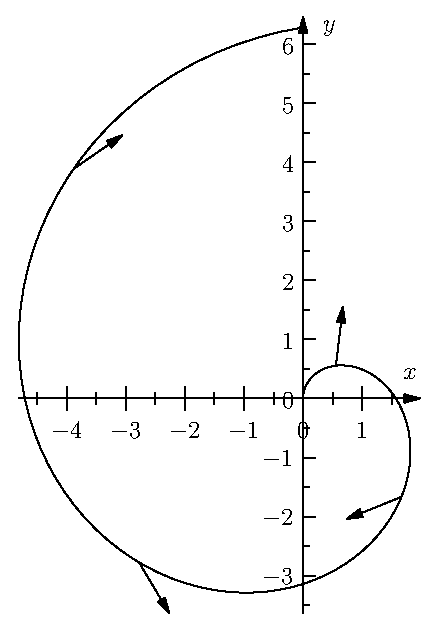
\includegraphics{./cap_curvas/figs/espiral}
\end{resp}

\begin{exer} Um erro comum entre estudantes é substituir a definição de vetor binormal unitário $\vec{B}=\vec{T}\times\vec{N}$ pela expressão espúria dada por $$\frac{\frac{d\vec{N}}{dt}}{\left\|\frac{d\vec{N}}{dt}\right\|}.$$ Calcule esta expressão para o movimento circular uniforme e verifique que ela é igual a $-\vec{T}$ e, portanto, perpendicular a $\vec{B}$.
\end{exer}

\begin{exer}
  Considere a curva $\vec{r}(t)$ definida no exercício E \ref{exe_co_arc5}. Obtenha o triedro de Frenet-Serret  $\vec{T}=\frac{2}{\sqrt{6+18t^3}}\vec{i}+\frac{-1+3t^{3/2}}{\sqrt{6+18t^3}}\vec{j}+\frac{1+3t^{3/2}}{\sqrt{6+18t^3}}\vec{k}$, $\vec{N} = \frac{-2t^{3/2}}{\sqrt{6+18t^3}}\vec{i}+\frac{1+t^{3/2}}{\sqrt{6+18t^3}}\vec{j}+\frac{1-t^{3/2}}{\sqrt{6+18t^3}}\vec{k}$ e $\vec{B} = -\frac{\vec{i}}{\sqrt{3}} - \frac{\vec{j}}{\sqrt{3}} + \frac{\vec{k}}{\sqrt{3}}$.
\end{exer}


\begin{exer}
Represente graficamente o terno de vetores $\vec{T}$,$\vec{N}$ e $\vec{B}$ e verifique através da regra da mão direita as seguintes identidades:
\begin{itemize}
\item[a)]$\vec{B}=\vec{T}\times\vec{N}$
\item[b)]$\vec{T}=\vec{N}\times\vec{B}$
\item[c)]$\vec{N}=\vec{B}\times\vec{T}$
\end{itemize}
Use a identidade vetorial dada por
$$\vec{u}\times\left(\vec{v}\times\vec{w}\right)=\vec{v}\left(\vec{u}\cdot\vec{w}\right)-\vec{w}\left(\vec{u}\cdot\vec{v}\right)$$ para obter as identidades $b$ e $c$ a partir de $a$.

[{\it Dica: Use o fato que $\vec{T}\cdot\vec{T}=\vec{N}\cdot\vec{N}=\vec{B}\cdot\vec{B}=1$ e
$\vec{T}\cdot\vec{N}=\vec{T}\cdot\vec{B}=\vec{N}\cdot\vec{B}=0$.}

\end{exer}
\begin{exer}
Considere a trajetória dada pela equações paramétricas
\begin{eqnarray*}
x&=&t\sin (t)\\
y&=&t\cos (t)\\
z&=&0
\end{eqnarray*}
Esboce gráfico dessa trajetória para $0\leq t \leq 2\pi$, indicando os pontos inicial e final. Esboce o triedro $\vec{T}$, $\vec{N}$ e $\vec{B}$ no instante $t=\pi/2$.(Obs.: Não é necessário calcular analiticamente o triedro.) Considere a identidade vetorial $\frac{d r^2}{dt}=2\vec{r}\cdot\frac{d\vec{r}}{dt}$ no instante $t=\pi/2$, ela é compatível com seu desenho?
\end{exer}
\begin{resp}
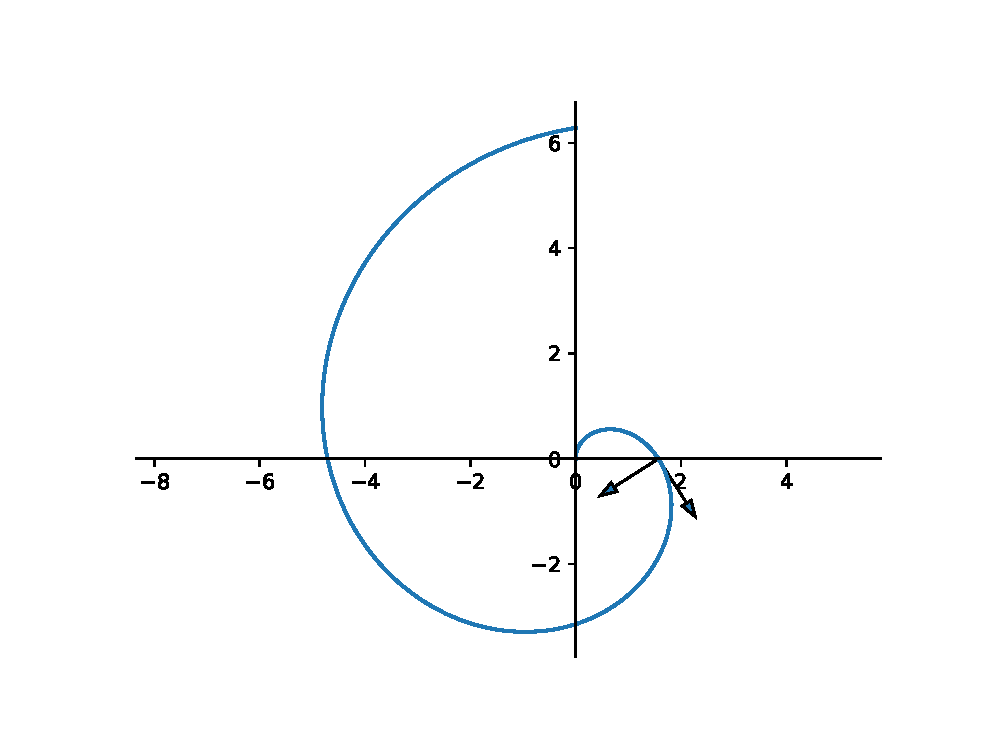
\includegraphics[scale=.8]{./cap_curvas/figs//espiral_lista_a1} 
Para o comentário sobre a derivada da norma ao quadrado, observe que $r^2=t^2$, assim:
\begin{eqnarray*}
\vec{r}\cdot\frac{d\vec{r}}{dt}=\frac{1}{2}\frac{d r^2}{dt}=t>0
\end{eqnarray*}
Em $t=\pi/2$, $\vec{r} = \frac{\pi}{2}\vec{i}$, isso é compatível com o fato de que a tangente tem componente positivo nessa direção (não é paralelo ao eixo y como na circunferência).
\end{resp}

\section{Curvatura e Torção}

Nessa seção, estamos interessados em definir, a cada ponto da curva, funções que medem o quanto ela está torcida ou curvada, isto é, se a curva é muito diferente de uma reta ou se está fora de qualquer plano do espaço. Primeiro, definiremos uma função chamada de curvatura\index{curvatura}, que mede a cada ponto do domínio, a norma da variação do vetor tangente com respeito ao comprimento de arco $s$. Naturalmente, queremos que a reta tenha curvatura nula, pois ela não difere da sua tangente em ponto algum. Para facilitar a visualização, podemos começar pensando apenas nas curvas que estão contidas em algum plano. A figura \ref{curvatura} apresenta uma noção de curvatura em um ponto.


\begin{figure}
\begin{center}
    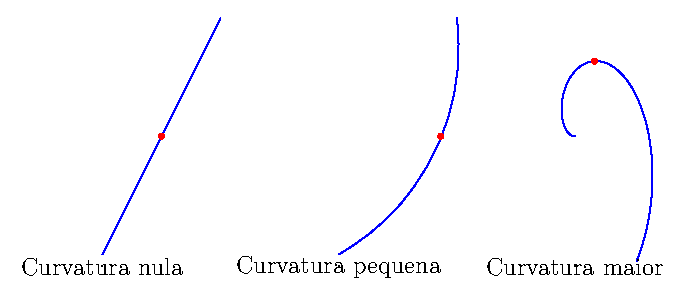
\includegraphics{./cap_curvas/figs/exemplos_de_curvatura2}
 \caption{Noção de curvatura em um ponto.\label{curvatura}}
  \end{center}
\end{figure}

O vetor normal $\vec{N}$,  sendo paralelo a $\frac{d\vec{T}}{dt}$ por definição, também é paralelo a $\frac{d\vec{T}}{ds}$, onde $s$ é comprimento do arco definido pela curva da trajetória de $\vec{r}(t)$. Assim, 
\begin{equation}{\label{Frenet_1}}
\frac{d \vec{T} }{ds}=\kappa   \vec{N},
\end{equation}
onde $\kappa(t)>0$ é uma função escalar chamada de curvatura. Por outro lado, calculamos a variação do vetor tangente com respeito ao comprimento de arco $s$ usando a regra da cadeia
$$
\frac{d \vec{T} }{ds}=\frac{d \vec{T} }{dt}\frac{dt}{ds}=\frac{d \vec{T} }{dt}\frac{1}{|s'(t)|},
$$
onde $s(t)$ é a função que mede o comprimento do arco dado pela expressão (\ref{defcomparco_1}). Usando o fato que\footnote{Teorema Fundamental do Cálculo, parte 2} $s'(t)=\left\|\frac{d\vec{r}(t)}{dt}\right\|$, temos:
$$
\frac{d \vec{T} }{ds}=\frac{1}{\|\frac{d\vec{r}(t)}{dt} \|}\frac{d \vec{T} }{dt}.
$$
Portanto, podemos escrever
$$
\kappa(t)=\frac{\|\frac{d\vec{T}(t)}{dt}\|}{\|\frac{d\vec{r}(t)}{dt}\|}.
$$

Definimos também, para cada ponto $t$ do domínio, o raio de curvatura\index{raio de curvatura} $\rho(t)$ da forma:
$$
\rho(t)=\frac{1}{\kappa(t)}.
$$
O raio de curvatura tem a seguinte interpretação geométrica: considere um ponto $\vec{r}(t_0)$ onde da curvatura não é nula e defina o ponto $\vec{r}(t_0)+\kappa(t_0)\vec{N}$, chamado de centro de curvatura\index{centro de curvatura}. O círculo centrado no centro de curvatura e raio $\rho(t_0)$ é tangente a curva em $t_0$ e possui a mesma curvatura (veja a figura \ref{raio_de_curvatura}).


\begin{figure}
\begin{center}
    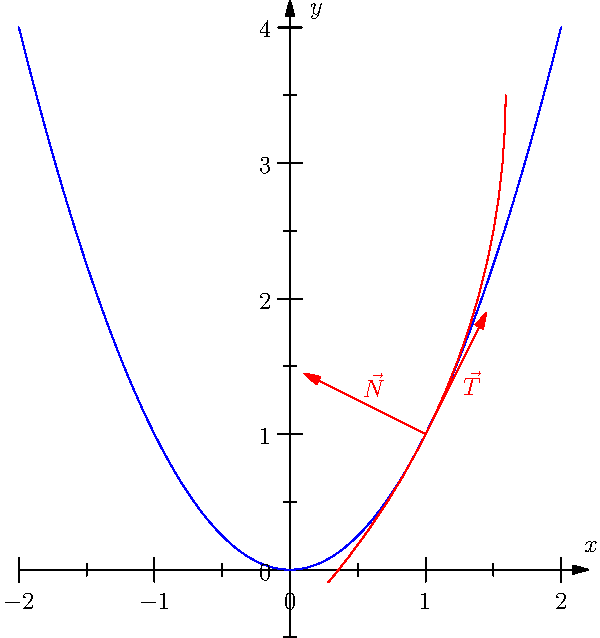
\includegraphics{./cap_curvas/figs/circulo_curvatura_parabola}
 \caption{Círculo de curvatura}\label{raio_de_curvatura}
  \end{center}
\end{figure}

\begin{ex}A curva descrita por $\vec{r}=a\cos(t)\vec{i}+a\sin(t)\vec{j},\qquad a>0,\ 0\leq t\leq 2\pi$ é uma cincunferência. Sua curvatura pode ser obtida da seguinte forma:
\begin{eqnarray}
\frac{d \vec{r}(t)}{dt}&=&-a\sin(t)\vec{i}+a\cos(t)\vec{j},\\
\left\|\frac{d\vec{r}(t)}{dt}\right\|&=&\sqrt{a^2\sin^2(t)+a^2\cos^2(t)}=\sqrt{a^2}=|a|=a,\\
 \vec{T}(t)&=&\frac{-a\sin(t)\vec{i}+a\cos(t)\vec{j}}{a}=-\sin(t)\vec{i}+\cos(t)\vec{j},\\
\end{eqnarray}

\end{ex}
\begin{ex}Dada a curva $y=x^2$, vamos encontrar a curvatura e o raio de curvatura no ponto $x=1$. Primeiro, encontramos uma parametrização para essa curva, por exemplo, $\vec{r}=t\vec{i}+t^2\vec{j}$. Calculamos:
$$
\frac{d\vec{r}(t)}{dt}=\vec{i}+2t\vec{j},
$$
$$
\left\|\frac{d\vec{r}(t)}{dt}\right\|=\sqrt{1+4t^2},
$$
$$
\vec{T}(t)=\frac{1}{\sqrt{1+4t^2}}\left(\vec{i}+2t\vec{j}\right)
$$
e
$$
\frac{d\vec{T}(t)}{dt}=-\frac{4t}{\sqrt{(1+4t^2})^3}\vec{i}+\left(-\frac{8t^2}{\sqrt{(1+4t^2})^3}+\frac{2}{\sqrt{1+4t^2}}\right)\vec{j},
$$
Em $t=1$, temos:
$$
\left\|\frac{d\vec{r}(t)}{dt}\right\|=\sqrt{5},
$$
$$
\frac{d\vec{T}(t)}{dt}=-\frac{4}{\sqrt{5^3}}\vec{i}+\left(-\frac{8}{\sqrt{5^3}}+\frac{2}{\sqrt{5}}\right)\vec{j}=-\frac{4}{\sqrt{5^3}}\vec{i}+\frac{2}{\sqrt{5^3}}\vec{j},
$$
e
$$
\left\|\frac{d\vec{T}(t)}{dt}\right\|=\sqrt{\frac{16}{5^3}+\frac{4}{5^3}}=\frac{2}{5}.
$$
Portanto,
$$
\kappa(1)=\frac{\|\frac{d\vec{T}}{dt}\|}{\|\frac{d\vec{r}}{dt}\|}=\frac{2}{5\sqrt{5}}
$$
e
$$
\rho(1)=\frac{5\sqrt{5}}{2}.
$$
veja representação geométrica na figura \ref{raio_de_curvatura}.
\end{ex}

O leitor deve ter observado que conhecendo somente a curvatura não é possível reconstruir uma curva a partir de um ponto dado. Um curva pode não estar contida em plano algum no espaço e, por isso, precisamos definir uma função escalar, chamada torção, que mede a magnitude da variação do vetor binormal. A figura \ref{torcao} apresenta uma ideia de torção\index{torção}: uma curva contida em algum plano no espaço tem torção nula e quando maior a variação com respeito ao plano definido por $\vec{T}$ e $\vec{N}$, maior a torção. O leitor deve tomar cuidado na interpretação da figura \ref{torcao}, pois se esticarmos indefinidamente a hélice circular representada, ela voltará a se aproximar de uma reta, que tem torção nula (veja problema \ref{prob_torcao}). Sabendo que a torção será definida em termos da variação do vetor binormal com respeito ao comprimento de arco $s(t)$, fazendo algumas observações:
$$
\frac{d\vec{B}}{ds}=\frac{d}{ds}\left(\vec{T}\times\vec{N}\right)=\frac{d\vec{T}}{ds}\times \vec{N}+\vec{T}\times\frac{d\vec{N}}{ds}.
$$
Usando a expressão (\ref{Frenet_1}), temos que $\frac{d\vec{T}}{ds}=\kappa\vec{N}$, logo 
$$
\frac{d\vec{B}}{ds}=\vec{T}\times\frac{d\vec{N}}{ds}.
$$
Isso implica que $\frac{d\vec{B}}{ds}$ é ortogonal a $\vec{T}$. Mas, pelo teorema \ref{teodernormacst}, temos que $\frac{d\vec{B}}{ds}$ é ortogonal a $\vec{B}$. Logo, $\frac{d\vec{B}}{ds}$ é paralelo a $\vec{N}$, ou seja, podemos definir
\begin{equation}{\label{Frenet_2}}
\frac{d\vec{B}}{ds}=-\tau\vec{N},
\end{equation}
onde $\tau$ é chamado de torção\index{torção}. O sinal negativo tem um propósito: quando $\tau>0$, $\frac{d\vec{B}}{ds}$ está no sentido de $-\vec{N}$; então se $P$ é um ponto sobre a curva movendo-se no sentido positivo, $\vec{B}$ gira em torno de $\vec{T}$ como um parafuso de rosca direita sendo apertado (veja a figura \ref{Curvatura_torcao_1}). Em alguns contextos, calculamos a módulo da torção, dada por
$$
|\tau|=\left\|\frac{d\vec{B}}{ds}\right\|=\frac{\|\frac{d\vec{B}(t)}{dt}\|}{\|\frac{d\vec{r}(t)}{dt}\|}.
$$


\begin{figure}
\begin{center}
    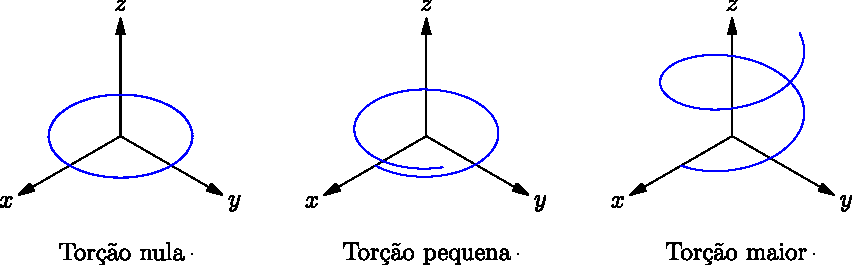
\includegraphics{./cap_curvas/figs/exemplos_de_torcao}
 \caption{Ideia de torção.}\label{torcao}
  \end{center}
\end{figure}



Ainda, definimos o raio de torção\index{raio de torção} por
$$
\sigma(t)=\frac{1}{\tau(t)}.
$$

Podemos calcular $\frac{d\vec{N}}{ds}$ em termos da curvatura e da torção:
\begin{equation*}
\frac{d\vec{N}}{ds}=\frac{d}{ds}\left(\vec{B}\times\vec{T}\right)=\frac{d\vec{B}}{ds}\times \vec{T}+\vec{B}\times\frac{d\vec{T}}{ds}.
\end{equation*}
Usando as expressões (\ref{Frenet_1}) e (\ref{Frenet_2}), escrevemos
\begin{equation*}
\frac{d\vec{N}}{ds}=-\tau\vec{N} \times \vec{T}+\vec{B}\times \kappa \vec{N}.
\end{equation*}
ou seja,
\begin{equation}{\label{Frenet_3}}
\frac{d\vec{N}}{ds}=-\kappa \vec{T}+\tau \vec{B}.
\end{equation}
As equações (\ref{Frenet_1}), (\ref{Frenet_2}) e (\ref{Frenet_3}) são chamadas de Fórmulas de Frenet-Serret.

Como esperávamos, se $\kappa=0$, então $\frac{d\vec{T}}{ds}=\vec{0}$, o que implica que $\vec{T}$ não varia ao longo da curva, ou seja, a curva é uma reta. Agora, se $\tau=0$, então $\frac{d\vec{B}}{ds}=\vec{0}$ e $\vec{B}$ é um vetor constante. Como $\vec{B}\cdot \vec{T}=\vec{B}\cdot \frac{d\vec{r}}{ds}=0$, então podemos integrar para obter $\vec{B}\cdot (\vec{r}-\vec{r_0})=0$, onde $r_0$ é um vetor constante da integração. Logo $\vec{r}$ está contido no plano ortogonal a $\vec{B}$.



\begin{ex} Vamos calcular curvatura, raio de curvatura e o módulo da torção para a hélice circular $\vec{r}(t)=\cos(t)\vec{i}+\sin(t)+t\vec{k}$:
$$
\frac{d\vec{r}(t)}{dt}=-\sin(t)\vec{i}+\cos(t)+\vec{k},
$$
$$
\left\|\frac{d\vec{r}(t)}{dt}\right\|=\sqrt{2},
$$
$$
\vec{T}(t)=-\frac{\sin(t)}{\sqrt{2}}\vec{i}+\frac{\cos(t)}{\sqrt{2}}+\frac{1}{\sqrt{2}}\vec{k},
$$
$$
\frac{d\vec{T}(t)}{dt}=-\frac{\cos(t)}{\sqrt{2}}\vec{i}-\frac{\sin(t)}{\sqrt{2}},
$$
$$
\left\|\frac{d\vec{T}(t)}{dt}\right\|=\frac{1}{\sqrt{2}},
$$
$$
\kappa(t)=\frac{1}{\sqrt{2}}\cdot \frac{1}{\sqrt{2}}=\frac{1}{2},
$$
$$
\rho(t)=2,
$$
$$
\vec{N}(t)=-\cos(t)\vec{i}-\sin(t)\vec{j},
$$
\begin{eqnarray*}
\vec{B}(t)&=&\left|\begin{array}{ccc}\vec{i}&\vec{j}&\vec{k}\\-\frac{\sin(t)}{\sqrt{2}}&\frac{\cos(t)}{\sqrt{2}}&\frac{1}{\sqrt{2}}\\-\cos(t)&-\sin(t)&0\end{array}\right|\\
&=&\frac{\sin(t)}{\sqrt{2}}\vec{i}-\frac{\cos(t)}{\sqrt{2}}\vec{j}+\frac{1}{\sqrt{2}}\vec{k}.
\end{eqnarray*}
$$
\frac{d\vec{B}(t)}{dt}=\frac{\cos(t)}{\sqrt{2}}\vec{i}+\frac{\sin(t)}{\sqrt{2}}\vec{j},
$$
$$
\left\|\frac{d\vec{B}(t)}{dt}\right\|=\frac{1}{\sqrt{2}},
$$
$$
|\tau(t)|=\frac{1}{2}.
$$
\end{ex}

\begin{exer} Calcule a curvatura, o raio de curvatura e o módulo da torção das curvas abaixo:
\begin{itemize}
\item[a)] $\vec{r}=a\cosh(t)\vec{i}+b\sinh(t)\vec{j}$, $-\infty<t<\infty$, $a>0,\ b>0$.
\item[b)] $\vec{r}=a\cos(t)\vec{i}+b\sin(t)\vec{k}$, $0\leq t\leq 2\pi$, $a>0,\ b>0$.
\item[c)] $\vec{r}=a\cos(t)\vec{i}+a\sin(t)+ct\vec{k}$, $t\geq 0$, $a>0,\ c>0$.

\end{itemize}
\end{exer}
 
 \begin{exer}{\label{prob_torcao}} Dada a hélice circular $\vec{r}=a\cos(t)\vec{i}+a\sin(t)+ct\vec{k}$, $t\geq 0$, $a>0,\ c>0$, calcule o valor de $c$ para que a torção seja máxima.
 \end{exer}


 
 \begin{figure}
\begin{center}
    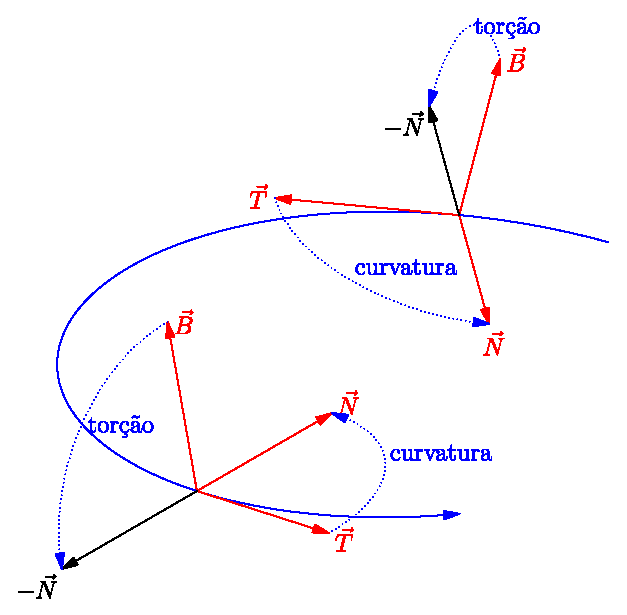
\includegraphics{./cap_curvas/figs/curvatura_torcao}
 \caption{Curvatura e Torção}\label{Curvatura_torcao_1}
  \end{center}
\end{figure}


A curvatura e a torção podem ser calculadas de maneira mais simples. Para concluir isso, começamos calculando as derivadas de $\vec{r}$. Usamos aqui que $s'(t)=\left\|\frac{d\vec{r}(t)}{dt}\right\|$, obtida da equação (\ref{defcomparco_1}):
$$
\frac{d\vec{r}}{dt}=\frac{d\vec{r}}{ds}\frac{ds}{dt}=s' \vec{T},
$$
\begin{eqnarray*}
\frac{d^2\vec{r}}{dt^2}&=&s'' \vec{T}+s' \frac{d\vec{T}}{dt}\\&=&s'' \vec{T}+s' \|\frac{d\vec{T}}{dt}\|\vec{N}\\
&=&s'' \vec{T}+(s')^2 \kappa \vec{N}
\end{eqnarray*}
e
\begin{eqnarray*}
\frac{d^3\vec{r}}{dt^3}&=&s''' \vec{T}+s''\frac{d\vec{T}}{dt}+2s's''\kappa \vec{N}+s'^2 \left(\kappa \frac{d\vec{N}}{dt}+\kappa' \vec{N}\right)\\
&=&s''' \vec{T}+s''s'\kappa \vec{N}+\left(2s's''\kappa+s'^2\kappa'\right) \vec{N}\\
&+&s'^3 \kappa (-\kappa \vec{T}+\tau\vec{B})\\
&=&\left(s'''-\kappa^2s'^3\right) \vec{T}+\left(3s''s'\kappa +s'^2\kappa'\right)\vec{N}+s'^3 \kappa \tau\vec{B},
\end{eqnarray*}
onde usamos as expressões (\ref{Frenet_1}) e (\ref{Frenet_3}). Agora, tomamos os seguintes produtos:
$$
\frac{d\vec{r}}{dt} \times \frac{d^2 \vec{r}}{dt^2}=s'^3\kappa \vec{B}\qquad\text{e}\qquad
\frac{d\vec{r}}{dt} \times \frac{d^2\vec{r}}{dt^2} \cdot \frac{d^3\vec{r}}{dt^3}=s'^6\kappa^2\tau.
$$
Isso implica em 
$$
\left\|\frac{d\vec{r}}{dt} \times \frac{d^2\vec{r}}{dt^2}\right\|=|s'|^3\kappa\qquad\text{e}\qquad
\frac{d\vec{r}}{dt} \times \frac{d^2\vec{r}}{dt^2} \cdot \frac{d^3 \vec{r}}{dt^3}=\left\|\frac{d\vec{r}}{dt} \times \frac{d^2\vec{r}}{dt^2}\right\|^2\tau.
$$
ou seja,
\begin{equation}{\label{curvatura_2}}
\kappa =\frac{\|\frac{d\vec{r}}{dt} \times \frac{d^2 \vec{r}}{dt^2}\|}{\|\frac{d\vec{r}}{dt}\|^3}
\end{equation}
e
\begin{equation}{\label{torcao_2}}
\tau=\frac{\frac{d\vec{r}}{dt} \times \frac{d^2 \vec{r}}{dt^2} \cdot \frac{d^3 \vec{r}}{dt^3} }{\|\frac{d\vec{r}}{dt} \times \frac{d^2\vec{r}}{dt^2}\|^2}.
\end{equation}

\begin{obs}\index{aceleração!normal}\index{aceleração!tangencial}Uma aplicação natural é a decomposição da aceleração em suas componentes tangencial e normal. Observe que
$$
\frac{d\vec{r}}{dt}=\vec{v}=v\vec{T}=s' \vec{T}
$$
e
$$
\vec{a}=v' \vec{T}+v^2 \kappa \vec{N}.
$$
Concluímos que a aceleração está no plano normal a $\vec{B}$ e possui componentes tangencial e normal:
$$
\vec{a}=a_T \vec{T}+a_N \vec{N},
$$
onde $a_T=v'$ e $a_N=v^2\kappa$. Então, se a velocidade possui normal constante, temos que $v'=0$ e a aceleração possui apenas componente normal.

\end{obs}

\begin{ex} Consideramos a elipse no plano $xy$ cuja equação canônica é dada por:
  $$\frac{x^2}{a^2} + \frac{y^2}{b^2} = 1. $$
  Aqui $a$ e $b$ são constantes positivas e representam os comprimetos dos semieixos da elipse.
  Inserimos a parametrização $x(t)=a\cos(t)$ e $y(t)=b\sin(t)$ para obter o vetor $\vec{r}(t)$:
  $$\vec{r}(t) = a\cos(t)\vec{i} + b\sin(t)\vec{j}.$$
  as derivadas de $\vec{r}(t)$ são, portanto, dadas por:
$$r'(t)=-a\sin(t)\vec{i}+b\cos(t)\vec{j}$$  
$$r''(t)=-a\cos(t)\vec{i}-b\sin(t)\vec{j}$$
Assim, temos:
\begin{eqnarray*}\vec{r}'(t)\times\vec{r}''(t)&=&\left(-a\sin(t)\vec{i}+b\cos(t)\vec{j}\right)\times\left(-a\cos(t)\vec{i}-b\sin(t)\vec{j}\right)\\
&=&ab\sin^2(t)\vec{k}+ab\cos^2(t)\vec{k}=ab\vec{k}
\end{eqnarray*}
Onde usamos a identidade trigonométrica $\sin^2(t)+\cos^2(t)=1$ e as identidades vetoriais $\vec{i}\times\vec{j}=\vec{k}$, $\vec{j}\times\vec{i}=-\vec{k}$  e $\vec{i}\times\vec{i}=\vec{j}\times\vec{j}=\vec{0}$.
Agora calculamos $\|\vec{r}(t)\|$:
$$\|\vec{r}(t)\|=\left[a^2\sin^2(t)+b^2\cos^2(t)\right]^{1/2}$$

Desta forma, temos:
$$\kappa(t)=\frac{\|r'(t)\times r''(t)\|}{\|r'(t)\|^3}=\frac{ab}{\left[a^2\sin^2(t)+b^2\cos^2(t)\right]^{3/2}}$$
Vale observar que os pontos de máxima e mínima curvatura estão nos vértices, isto é, $t=0$, $t=\frac{\pi}{2}$, $t=\pi$ e $t=\frac{3\pi}{2}$. A prova dessa afirmação será objeto de exercício.

Podemos expressão a curvatura da elipse em termos das variáveis originais $x$ e $y$:
\begin{eqnarray*}
\kappa(x, y)&=&\frac{ab}{\left(\frac{a^2}{b^2}y^2+\frac{b^2}{a^2}x^2\right)^{3/2}}\\
\kappa(x)&=&\frac{ab}{\left(a^2+\left(\frac{b^2-a^2}{a^2}\right)x^2\right)^{3/2}}\\
\kappa(y)&=&\frac{ab}{\left(b^2+\left(\frac{a^2-b^2}{b^2}\right)y^2\right)^{3/2}}\\
\end{eqnarray*}


\end{ex} 


\begin{ex} Consideremos agora, a curva gerada pelas seguintes equações paramétricas:
$$x(t)=\cos(t)\qquad y(t)=\sin(t)\qquad z(t)=f(t).$$
 Onde $f(t)$ é uma função dada. Observe que a projeção desta curva no plano $xy$ é uma circuferência de raio 1. A curva é, portanto, gerada pela trajetória de ponto cuja projeção do movimento no plano $xy$ é cirvular e a altura é dada pela função $f(t)$. Podemos calcular a curvatura e a torção conforme a seguir:
 \begin{eqnarray*}
  \vec{r}(t)&=&\cos(t)\vec{i}+\sin(t)\vec{j}+f(t)\vec{k}\\
  \frac{d\vec{r}}{dt}&=&-\sin(t)\vec{i}+\cos(t)\vec{j}+f'(t)\vec{k}\\
  \frac{d^2\vec{r}}{dt^2}&=&-\cos(t)\vec{i}-\sin(t)\vec{j}+f''(t)\vec{k}\\
  \frac{d^3\vec{r}}{dt^3}&=&\sin(t)\vec{i}-\cos(t)\vec{j}+f'''(t)\vec{k}
 \end{eqnarray*}
Assim, calculamos:
 \begin{eqnarray*}
  \frac{d\vec{r}}{dt} \times \frac{d^2 \vec{r}}{dt^2} &=&\left[f''(t)\cos(t)+f'(t)\sin(t)\right]\vec{i}+\left[-f'(t)\cos(t)+f''(t)\sin(t)\right]\vec{j}+\vec{k}\\
\frac{d \vec{r}}{dt} \times \frac{d^2\vec{r}}{dt^2} \cdot \frac{d^3\vec{r}}{dt^3} &=&f'(t)+f'''(t)\\
 \left\|\frac{d\vec{r}}{dt} \times\frac{d^2\vec{r}}{dt^2}\right\|&=&\sqrt{1+\left(f'(t)\right)^2+\left(f''(t)\right)^2}\\
 \left\|\frac{d\vec{r}}{dt}\right\|&=&\sqrt{1+\left(f'(t)\right)^2}
 \end{eqnarray*}
E finalmente, obtemos:
 \begin{eqnarray*}
\kappa&=&\frac{\sqrt{1+\left(f'(t)\right)^2+\left(f''(t)\right)^2}}{\left({1+\left(f'(t)\right)^2}\right)^{3/2}}\\
\tau&=&\frac{f'(t)+f'''(t)}{1+\left(f'(t)\right)^2+\left(f''(t)\right)^2}
 \end{eqnarray*}
Podemos, agora, explorar diversos casos particulares:
\begin{itemize}
 \item [a)] Caso $f(t)=c$ constante. Neste caso, recaímos na circunferência de raio 1, cuja curvatura é 1 e a torção é nula.
 \item [b)] Caso $f(t)=ct$ com $c$ constante. Recaímos na hélice cicular uniforme, já estudada, cuja curvatura é $\frac{1}{1+c^2}$ e a torção é $\frac{c}{1+c^2}$.
 \item [c)] Caso $f(t)=ct^2$ com $c$ constante. Recaímos na hélice cicular com espaçamento linearmente crescente, cuja curvatura é dada por ${\frac {\sqrt {4\,{c}^{2}+1+4\,{c}^{2}{t}^{2}}}{ \left( 1+4\,{c}^{2}{t
}^{2} \right) ^{3/2}}}$ e cuja torção é dada por $2\,{\frac {ct}{4\,{c}^{2}+1+4\,{c}^{2}{t}^{2}}}$.
 \item [d)] Caso $f(t)=\sin(t)$. Recaímos na elipse de semieixos $1$ e $\sqrt{2}$ no plano $y=z$. Neste caso, a curvatura é $\kappa=\frac{\sqrt{2}}{\left(1+\cos(t)^2\right)^{3/2}}$ e a torção é nula.
 \item [e)] Caso $\tau=0$, isto é, $f'(t)+f'''(t)=0$, o que é equivalente a $f(t)=a+b\cos(t)+c\sin(t)$ onde $a$, $b$ e $c$ são constantes. Recaímos na elipse de semieixos $1$ e $\sqrt{1+b^2+c^2}$ no plano $z=bx+cy$. Neste caso, a curvatura é $\kappa={\frac {\sqrt {b^2+c^2+1}}{\left(1-bc\sin(2t)+c^2\cos^2(t)+b^2\sin^2(t) \right) ^{3/2}}}$ e a torção é nula.
  \end{itemize}
\end{ex}


\subsection*{Exercícios resolvidos}

\begin{exeresol}
Considere a hélice dada por
\begin{eqnarray*}
x&=&a\cos(wt)\\
y&=&a\sin(wt)\\
z&=&ct.\\
\end{eqnarray*}
Onde $a$ e $w$ são constantes positivas.
\begin{itemize}
\item[a)] Encontre  a curvatura desta hélice usando a fórmula
$$\kappa=\frac{\left\|\vec{r}\ \!'(t)\times \vec{r}\ \!''(t)\right\|}{\|r\ \!'(t)\|^3}.$$
\item[b)] Encontre o módulo da torção desta curva usando a seguinte fórmula para calcular o vetor binormal unitário: $$\vec{B}=\frac{\vec{r}\ \!'(t)\times \vec{r}\ \!''(t)}{\left\|\vec{r}\ \!'(t)\times \vec{r}\ \!''(t)\right\|}$$
e a seguinte fórmula para o módulo da torção:
$$|\tau|=\frac{\|B\ \!'(t)\|}{\|\vec{r}\ \!'(t)\|}=\left\|\frac{d\vec{B}}{ds}\right\|$$

\item[c)] Discuta o sinal da torção em função do sinal de $cw$. 
\item[d)] Confira a conclusão do item c), sabendo que $\vec{N}=-\cos(wt)\vec{i}-\sin(wt)\vec{j}$
\end{itemize}
\end{exeresol}
\begin{resol}
 Observe que:
\begin{eqnarray*}
\vec{r}(t)&=&a\cos(wt)\vec{i}+a\sin(wt)\vec{j}+ct\vec{k},\\
\vec{r}~\!'(t)&=&-aw\sin(wt)\vec{i}+aw\cos(wt)\vec{j}+c\vec{k},\\
\vec{r}~\!''(t)&=&-aw^2\cos(wt)\vec{i}-aw^2\sin(wt)\vec{j}.
\end{eqnarray*}
Assim:
\begin{eqnarray*}
\vec{r}~\!'(t)\times \vec{r}~\!''(t)&=&\left|
\begin{array}{ccc}
\vec{i}&\vec{j}&\vec{k}\\[0.5cm]
-aw\sin(wt)&aw\cos(wt)&c\\[0.5cm]
-aw^2\cos(wt)&-aw^2\sin(wt)&0
\end{array}
\right|\\
&=&
acw^2\sin(wt)\vec{i}-acw^2\cos(wt)\vec{j}+a^2w^3\underbrace{\left(\cos^2(wt)+\sin^2(wt)\right)}_{1}\vec{k}\\
&=&acw^2\sin(wt)\vec{i}-acw^2\cos(wt)\vec{j}+a^2w^3\vec{k}
\end{eqnarray*}
e
\begin{eqnarray*}
\|\vec{r}~\!'(t)\times \vec{r}~\!''(t)\|&=&\sqrt{a^2c^2w^4\sin^2(wt)+a^2c^2w^4\cos^2(wt)+a^4w^6}\\
&=&\sqrt{a^2c^2w^4+a^4w^6}=|a|w^2\sqrt{c^2+a^2w^2}=aw^2\sqrt{c^2+a^2w^2}
\end{eqnarray*}

Usamos a fórmula da curvatura:
\begin{eqnarray*}\kappa &=& \frac{\left\|\vec{r}'(t)\times \vec{r}''(t)\right\|}{\|r'(t)\|^3}\\
&=&\frac{aw^2\sqrt{c^2+a^2w^2}}{\left\|-aw\sin(wt)\vec{i}+aw\cos(wt)\vec{j}+c\vec{k}\right\|^3}\\
&=&\frac{aw^2\sqrt{c^2+a^2w^2}}{\left(a^2w^2+c^2\right)^{3/2}}\\
&=&\frac{aw^2}{{a^2w^2+c^2}}\\
\end{eqnarray*}


Agora usamos a fórmula da torção:
\begin{eqnarray*}\vec{B}&=&\frac{\vec{r}'(t)\times \vec{r}''(t)}{\left\|\vec{r}'(t)\times \vec{r}''(t)\right\|}\\
&=&\frac{acw^2\sin(wt)\vec{i}-acw^2\cos(wt)\vec{j}+a^2w^3\vec{k}}{|a|w^2\sqrt{c^2+a^2w^2}}\\
&=&\frac{ac\sin(wt)\vec{i}-ac\cos(wt)\vec{j}+a^2w\vec{k}}{a\sqrt{c^2+a^2w^2}}
\end{eqnarray*}

Sabemos que o módulo da torção é dado por:
\begin{eqnarray*}
|\tau|&=&\left\|\frac{d}{ds}\vec{B}\right\|\\
&=& \left\|\frac{d}{dt}\vec{B} \right\|/\|r'(t)\|\\
\end{eqnarray*}

\begin{eqnarray*}
 \frac{d}{dt}\vec{B} 
&=&\frac{acw\cos(wt)\vec{i}+acw\sin(wt)\vec{j}}{a\sqrt{c^2+a^2w^2}}
\end{eqnarray*}
e
\begin{eqnarray*}
\|r'(t)\|&=&\left\|-aw\sin(wt)\vec{i}+aw\cos(wt)\vec{j}+c\vec{k}\right\|\\
&=&\sqrt{c^2+a^2w^2}
\end{eqnarray*}


\begin{eqnarray*}
 \frac{d}{ds}\vec{B} 
&=&\frac{acw\cos(wt)\vec{i}+acw\sin(wt)\vec{j}}{a(c^2+a^2w^2)}
\end{eqnarray*}

Portanto:
\begin{eqnarray*}
|\tau|=\left\|\frac{d}{ds}\vec{B}\right\|&=&
\frac{|acw|}{a(c^2+a^2w^2)}\\
&=&\frac{|c|w}{{c^2+a^2w^2}}
\end{eqnarray*}
Observando a orientação da curva, vemos que a ela é dextrógira se $c>0$, levógira se $c<0$, o sinal da torção é o sinal de $c$:
\begin{eqnarray*}
\tau=\frac{cw}{{c^2+a^2w^2}}
\end{eqnarray*}

Podemos verificar essa conclusão sabendo que:
\begin{eqnarray*}
\tau&=&-\frac{d}{ds}\vec{B}\cdot\vec{N}\\
&=&-\left(\frac{acw\cos(wt)\vec{i}+acw\sin(wt)\vec{j}}{a(c^2+a^2w^2)}\right)\cdot\left(-\cos(wt)\vec{i}-\sin(wt)\vec{j}\right)\\
&=&\frac{cw\cos^2(wt)+cw\sin^2(wt)}{(c^2+a^2w^2)}\\
&=&\frac{cw}{c^2+a^2w^2}
\end{eqnarray*}

\end{resol}

\begin{exeresol}
Mostre que se $a_N$ e $a_T$ indicam as acelerações normal e tangencial, respectivamente, então
$$\|\vec{a}\|^2=a_N^2+a_T^2$$
onde $\vec{a}$ é o vetor aceleração. Verifique esta identidade na trajetória dada por
\begin{eqnarray*}
 \vec{r}(t)=3\cos (t) \vec{i} + 3\sin (t) \vec{j} +t^2\vec{k}.
\end{eqnarray*}
[{\it Dica: use o fato que $\|\vec{a}\|^2=\vec{a}\cdot\vec{a}$.}]
\end{exeresol}

\begin{resol}
Basta usar a seguinte identidade e simplifique:
\begin{eqnarray*}
 \|\vec{a}\|^2&=&\|a_T\vec{T}+a_N\vec{N}\|^2= \left(a_T\vec{T}+a_N\vec{N}\right)\cdot \left(a_T\vec{T}+a_N\vec{N}\right)
 \end{eqnarray*}
A trajetória em questão é dada por:
\begin{eqnarray*}\vec{r}(t)=3\cos (t) \vec{i} + 3\sin (t) \vec{j} +t^2\vec{k}
\end{eqnarray*}
Para obter os valores pedidos, calculamos:
\begin{eqnarray*}\vec{r}'(t)&=&-3\sin (t) \vec{i} + 3\cos (t) \vec{j} +2t\vec{k}\\
\vec{r}''(t)&=&-3\cos (t) \vec{i} - 3\sin (t) \vec{j} +2\vec{k}\\
\|\vec{r}'(t)\|&=&\left(9\sin^2(t)+9\cos^2(t)+4t^2\right)^{1/2}=\left(9+4t^2\right)^{1/2}
\end{eqnarray*}

\begin{eqnarray*}a_N=\frac{\|\vec{r}'(t)\times \vec{r}''(t)\|}{\|\vec{r}'(t)\|}
\end{eqnarray*}
onde
\begin{eqnarray*}\vec{r}'(t)\times \vec{r}''(t)&=&
\left|\begin{array}{ccc}
\vec{i}&\vec{j}&\vec{k}\\
-3\sin (t) & 3\cos (t) & 2t\vec{k}\\
-3\cos (t) & -3\sin (t) & 2\vec{k}
\end{array}
\right|\\&=&\left(6\cos(t)+6t\sin(t)\right)\vec{i}+\left(-6t\cos(t) +6\sin(t)\right)\vec{j}+\underbrace{\left(9\sin^2(t)+9\cos^2(t)\right)}_{9}\vec{k}
\end{eqnarray*}
Assim:
\begin{eqnarray*}
\left\|\vec{r}'(t)\times \vec{r}''(t)\right\|&=&\left[\left(6\cos(t)+6t\sin(t)\right)^2+\left(-6t\cos(t) +6\sin(t)\right)^2+81\right]^{1/2}\\
&=&\left[\left(36\cos^2(t)+72\sin(t)\cos(t) + 36t^2\sin^2(t)\right)\right.\\&+&\left.\left(36t^2\cos^2(t) -72 \cos(t)\sin(t) + 36 \sin^2(t)\right) + 81\right]^{1/2}\\
&=&\left[36+36t^2+81\right]^{1/2}=\left(117+36t^2\right)^{1/2}
\end{eqnarray*}
Portanto
\begin{eqnarray*}a_N=\frac{\left(117+36t^2\right)^{1/2}}{\left(9+4t^2\right)^{1/2}}
\end{eqnarray*}
e
\begin{eqnarray*}\kappa=\frac{\left(117+36t^2\right)^{1/2}}{\left(9+4t^2\right)^{3/2}}
\end{eqnarray*}

A aceleração tangencial pode ser obtida conforme
\begin{eqnarray*}a_T=\frac{\vec{v}\cdot \vec{a}}{v}=\frac{9\sin(t)\cos(t) -9\sin(t) \cos(t)+4t}{\left(9+4t^2\right)^{1/2}}=\frac{4t}{\left(9+4t^2\right)^{1/2}}.
\end{eqnarray*}

Agora, retornamos ao pedido nesta lista:
\begin{eqnarray*}
 \|\vec{a}\|^2&=&\left\|-3\cos (t) \vec{i} - 3\sin (t) \vec{j} +2\vec{k}\right\|^2\\&=&3^2+2^2=13.
\end{eqnarray*}
E também:
\begin{eqnarray*}
a_N^2+a_T^2&=&\left(\frac{\left(117+36t^2\right)^{1/2}}{\left(9+4t^2\right)^{1/2}}\right)^2+\left(\frac{4t}{\left(9+4t^2\right)^{1/2}}\right)^2\\
&=&\frac{117+36t^2}{9+4t^2}+\frac{16t^2}{9+4t^2}=\frac{117+52t^2}{9+4t^2}\\&=&1,
\end{eqnarray*}
o que verifica a identidade.
 
\end{resol}



\begin{exeresol}
Mostre que a curvatura do gráfico da função
$$y=f(x)$$
sobre o plano $xy$
é dada pela expressão
$$\kappa(x)=\frac{|f''(x)|}{\left(1+f'(x)^2\right)^{3/2}}.$$
Use esta expressão para obter a curvatura das seguintes curvas planas:
\begin{itemize}
\item[a)] $y=ax+b$
\item[b)]$y=\sqrt{a^2-x^2}$, $-a<x<a$ onde $a>0$.
\item[c)] $y=x^4$
\item[d)] $y=ax^2$ 
\item[e)] $y=\cosh(x)$
\item[f)] $y=\sinh(x)$
\item[g)] $y=\cos(x)$
\end{itemize}
Como você interpreta os casos a e b? As curvas dos ítens c e g possuem pontos onde a curvatura é zero. Que implicação isso tem sobre a existência do vetor normal unitário $\vec{N}$? Interprete geometricamente.


[{\it Dica.: Use a parametrização $\vec{r}=t\vec{i}+f(t)\vec{j}$ e aplique na expressão para a curvatura.}]
\end{exeresol}


\begin{resol}
  Use a parametrização:
 $$\vec{r}(t) = t\vec{i}+f(t)\vec{j}$$ na fórmula da curvatura dada por:
$$\kappa=\frac{\left\|\vec{r}'(t)\times \vec{r}''(t)\right\|}{\|r'(t)\|^3}=\frac{\left\|\left(\vec{i}+f'(t)\vec{j}\right)\times f''(t)\vec{j}~\!\right\|}{\|~\!\vec{i}+f'(t)\vec{j}\|^3}$$
e obtenha a expressão dada.


\begin{itemize}
\item[a)] $\kappa(x)=0$
\item[b)]$\kappa(x)=1/a$
\item[c)] $\kappa(x)=\frac{12x^2}{\left(1+16x^6\right)^{3/2}}$
\item[d)] $\kappa(x)=\frac{2|a|}{\left(1+4a^2x^2\right)^{3/2}}$ 
\item[e)] $\kappa(x)=\frac{1}{\cosh^2(x)}$
\item[f)] $\kappa(x)=\frac{\sinh(|x|)}{\left(1+\cosh^2(x)\right)^{3/2}}$
\item[g)] $\kappa(x)=\frac{\cos|x|}{\left(1+\sin^2(x)\right)^{3/2}}$
\end{itemize}

Obs.: A curva a) é uma reta, pelo que tem curvatura zero. A curva b) é uma semicircunferêcia de raio $a$, pelo que tem curvatura $1/a$. Nos pontos de curvatura zero, o vetor normal não está definido. 
No item c), $\lim_{x\to 0-}\vec{N}(t)=\lim_{x\to 0+}\vec{N}(t)=\vec{j}$, mas no item g), os limites não são iguais, evidenciando mudança de concavidade.


Para analisar mais rigorosamente a existência do vetor normal, observe que o vetor tangente e normal são dados por:
\begin{eqnarray*}
 \vec{T}(t)&=&\frac{\vec{r}~\!'(t)}{\|\vec{r}~\!'(t)\|}\\
 &=&\frac{\vec{i}+f'(t)\vec{j}}{\sqrt{1+f'(t)^2}}\\
 &=&\left(1+f'(t)^2\right)^{-1/2}\vec{i}+f'(t)\left(1+f'(t)^2\right)^{-1/2}\vec{j}
\end{eqnarray*}
\begin{eqnarray*}
 \vec{T}~\!'(t)
 &=&-f'(t)f''(t)\left(1+f'(t)^2\right)^{-3/2}\vec{i}\\
 &+&\left[f''(t)\left(1+f'(t)^2\right)^{-1/2}-f'(t)^2f''(t)\left(1+f'(t)^2\right)^{-3/2}\right]\vec{j}\\
 &=&\frac{f''(t)}{\left(1+f'(t)^2\right)^{3/2}}\left[-f'(t)\vec{i}+\vec{j}\right]\\
\vec{N}(t)&=&\frac{\vec{T}~\!'(t)}{\|\vec{T}~\!'(t)\|}\\
&=&\frac{f''(t)}{|f''(t)|}\frac{-f'(t)\vec{i}+\vec{j}}{\sqrt{1+f'(t)^2}}\\
&=&\text{sinal}\left(f''(t)\right)\frac{-f'(t)\vec{i}+\vec{j}}{\sqrt{1+f'(t)^2}}
\end{eqnarray*}
Já o vetor $\vec{B}(t)$ é dado por:
\begin{eqnarray*}
\vec{B}=\vec{T}\times \vec{N} &=& \frac{\vec{i}+f'(t)\vec{j}}{\sqrt{1+f'(t)^2}} \times \text{sinal}\left(f''(t)\right)\frac{-f'(t)\vec{i}+\vec{j}}{\sqrt{1+f'(t)^2}}\\
&=&\text{sinal}(f''(t))\frac{(1+f'(t)^2)\vec{k}}{1+f'(t)^2}\\
&=&\text{sinal}(f''(t))\vec{k}
\end{eqnarray*}

Alternativamente, do fato que $\vec{N}=\vec{B}\times \vec{T}$ e de o vetor $\vec{B}$ ser previsível por inspeção, poderíamos ter evitado os cálculos mais trabalhosos para obter o vetor $\vec{N}$:
$$\vec{N}=\left\{
\begin{array}{rr}
\vec{k}\times\vec{T},&f''(t)>0\\
-\vec{k}\times\vec{T},&f''(t)<0\\
\text{não definido},&f''(t)=0
\end{array}
\right.$$

O vetor $\vec{B}$ também poderia ter sido calculado pela fórmula:
 \begin{eqnarray*}
  \vec{B}&=&\frac{\vec{r}'(t)\times \vec{r}''(t)}{\left\|\vec{r}'(t)\times \vec{r}''(t)\right\|}
 \end{eqnarray*}
onde $$\vec{r}'(t)\times \vec{r}''(t)=\left(\vec{i}+f'(t)\vec{j}\right)\times f''(t)\vec{j}=f''(t)\vec{k}.$$

\end{resol}


\begin{exeresol}
Calcule o valor mínimo e o valor máximo do raio de curvatura de uma elipse de semi-eixos $a$ e $b$ quando $0<a<b$. 
Dica:
$$\kappa(t)=\frac{ab}{\left[a^2+(b^2-a^2)\cos^2(t)\right]^{3/2}}$$
e use o fato que $0\leq \cos^2(t) \leq1$. Faço o caso $a\leq b$ e $b \leq a$.

\begin{itemize}
 \item[a)] O que acontece quando $a=b$?
 \item[b)] Quais são os semi-eixos da elipse cujo raio de curvatura varia entre $50m$ e $400$m?
 \item[c)] Encontre os semi-eixos da elipse cuja curvatura máxima é $8m^{-1}$ e o semi-eixo menor é $\frac{1}{4}m$.
\end{itemize}
\end{exeresol}
\begin{resol}
As curvaturas máximas e mínimas são (não necessariamente respectivamente) $\frac{a}{b^2}$ e $\frac{b}{a^2}$. Os raios de curvatura associados são $\frac{b^2}{a}$ e $\frac{a^2}{b}$.
\begin{itemize}
 \item[a)] Quando $a=b$, a elipse é uma circunferência e o raio de curvatura é constante igual a $a$, que é o raio da circunferência.
\item[b)] Para calcular os semi-eixos da elipse cujo raio de curvatura varia entre $50m$ e $400$m, suponha, sem perda de generalidade, que $a<b$ e resolva:
 \begin{eqnarray*}
  \frac{a^2}{b} &=& 50\\
  \frac{b^2}{a} &=& 400\\
 \end{eqnarray*}
 Da primeira equação, temos $b=\frac{a^2}{50}$, o que substituimos na segunda equação para obter:
 \begin{eqnarray*}
   \frac{b^2}{a} &=& \frac{a^4}{50^2a}=400
 \end{eqnarray*}
o que significa
$$a^3=400\times 2500 = 1.000.000.$$
 Assim $a=100m$ e $b=\frac{a^2}{50}=200m$.
\item[c)] Sem perda de generalidade, considere $a<b$ e temos as equações:
  \begin{eqnarray*}\kappa_{max}=\frac{b}{a^2}=8\\
  \end{eqnarray*}
     Como $a=1/4$, obtemos:
     $b=8a^2=\frac{8}{16}=\frac{1}{2}m$.
 \end{itemize}


\end{resol}

\begin{exeresol}
Um automóvel se desloca com velocidade constante sobre uma pista cuja forma é uma elipse horizontal de semi-eixos $50m$ e $200m$. Calcule a velocidade do autómovel para que a aceleração normal máxima seja $2m/s^2$. 


\indent {\it Obs:} Para calcular a curvatura, você provavelmente usou uma parametrização do tipo $\vec{r}=a\sin (t) + b\cos (t)$, explique por que esta parametrização pode ser usada para obter a curvatura, mas não pode ser usada diretamente para calcular a aceleração normal.
\end{exeresol}
\begin{resol}
A curvatura máxima da pista é:
 $$k_{max}=\frac{200}{50^2}=\frac{2}{25}\text{m}^{-1}$$
 Sabemos que $a_N=\kappa v^2$, portanto a máxima velocidade possível é:
 $$v=\sqrt{\frac{a_N}{\kappa}}=5m/s$$

 Sobre a observação, a parametrização $\vec{r}=a\sin (t) + b\cos (t)$ descreve a elipse, mas não satisfaz a a condição de velocidade escalar constante, pelo que pode ser usada para obter a curvatura, mas não representa a cinética do problema.
\end{resol}
\begin{exer}
Considere a trajetória  dada por
$$x(t)=\cos(t),~~  y(t)=\sin 2t,~~ z(t)=0.$$

Esboce o gráfico desta trajetória sobre o plano $xy$. Encontre uma expressão para a curvatura $k$ como uma função da coordenada $x$ na forma $$\kappa(x)=\frac{|x|(6-4x^2)}{\left(5-17x^2+16x^4\right)^{3/2}}.$$ Mostre que a curvatura é zero na origem e apenas na origem. Esboce, agora, o gráfico da curvatura como função de $x$ abaixo do gráfico da curva.
Dica: Use identidades trigonométricas como $\sin(2t)=2\sin(t)\cos(t)$, $\cos(2t)=\cos^2(t)-\sin^2(t)$ e $\sin^2(t)+\cos^2(t)=1$.
\end{exer}
\begin{resol}
A curva é dada por:
$$\vec{r}(t)=\cos (t)\vec{i}+ \sin (2t)\vec{j}.$$
Assim:
 \begin{eqnarray*}
    \vec{r}~\!'(t)&=&-\sin(t)\vec{i}+ 2\cos(2t)\vec{j}\\
  \vec{r}~\!''(t)&=&-\cos (t)\vec{i}-4 \sin (2t)\vec{j}
 \end{eqnarray*}
 Portanto:
 \begin{eqnarray*}
  \|\vec{r}~\!'(t)\|&=&\sqrt{\sin^2(t)+4\cos^2(2t)}\\
  &=&\sqrt{\sin^2(t)+4-4\sin^2(2t)}\\
  &=&\sqrt{\sin^2(t)+4-16\sin^2(t)\cos^2(t)}\\
  &=&\sqrt{1-\cos^2(t)+4-16\left(1-\cos^2(t)\right)\cos^2(t)}\\
  &=&\sqrt{1-x^2+4-16(1-x^2)x^2}\\
  &=&\sqrt{5-17x^2+16x^4}
 \end{eqnarray*}
e
 \begin{eqnarray*}
    \vec{r}~\!'(t)\times \vec{r}~\!''(t)&=&\left(4\sin(t)\sin(2t)+2\cos(t)\cos(2t)\right)\vec{k}\\
 &=&\left[8\sin^2(t)\cos(t)+2\cos(t)\left(\cos^2(t)-\sin^2(t)\right)\right]\vec{k}\\
 &=&\left[6\sin^2(t)\cos(t)+2\cos^3(t)\right]\vec{k}\\
 &=&\left[6(1-x^2)x+2x^3\right]\vec{k}\\
 &=&\left[6x-4x^3\right]\vec{k}\\
  \end{eqnarray*}
  Portanto:
   \begin{eqnarray*}
    \|\vec{r}~\!'(t)\times \vec{r}~\!''(t)\|
 &=&|6x-4x^3|=|x|(6-4x^2)
  \end{eqnarray*}
e
$$\kappa(x)=\frac{|x|(6-4x^2)}{\left(5-17x^2+16x^4\right)^{3/2}}. $$

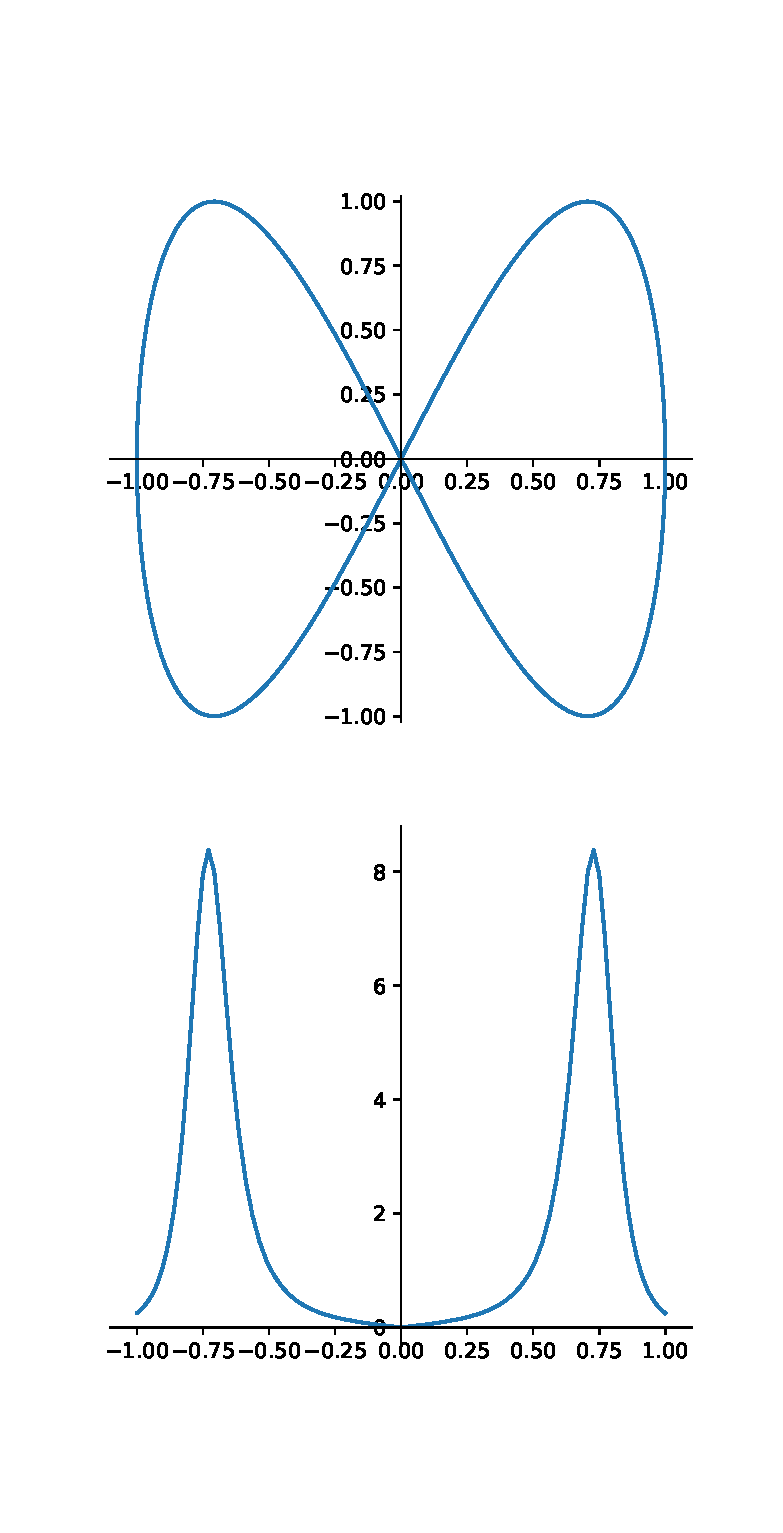
\includegraphics[scale=.6]{./cap_curvas/figs/lissa_lista_a1_2}
\end{resol}

\begin{exeresol}  Considere a hélice circular não uniforme dada por
  \begin{eqnarray*}
    x&=&\cos(t)\\
    y&=&\sin(t)\\
    z&=&f(t):=8\sqrt{t}.\\
  \end{eqnarray*}
  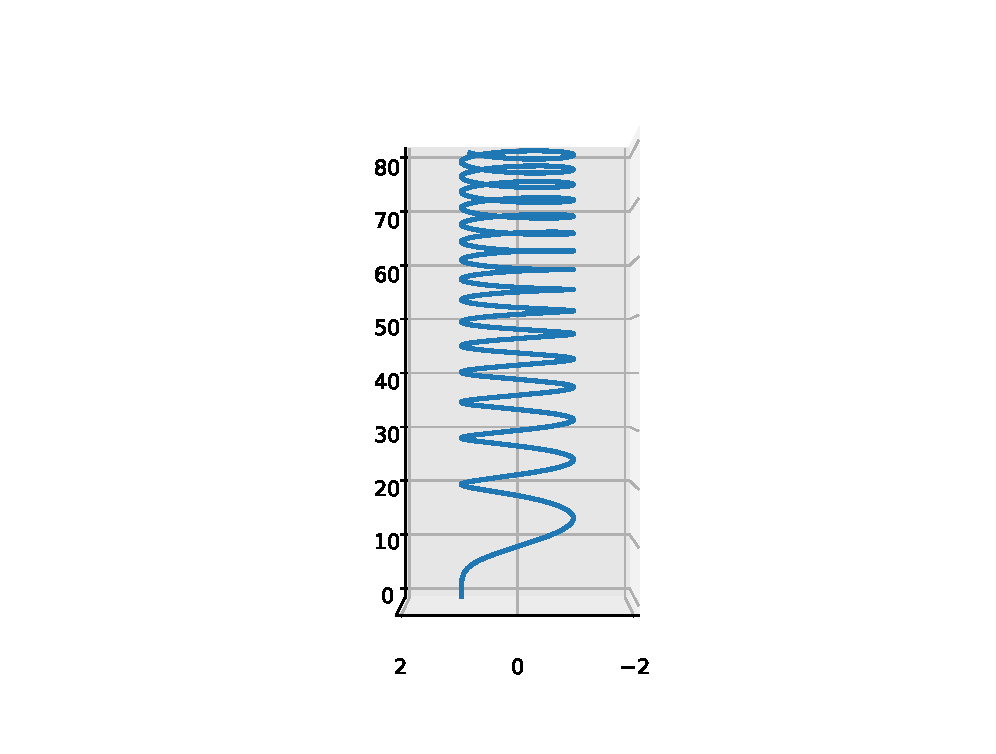
\includegraphics[scale=.6]{./cap_curvas/figs/helice_sqrt_z}
  \begin{itemize}
    \item[a)] Encontre o passo $P(t)$ (variação da coordenada $z$) entre os pontos dados por $t_0=t$ e $t_1=t+2\pi$ e mostre que $P(t)=\frac{2\pi}{\sqrt{8t} + \sqrt{8t+2\pi}}.$.
  \item[b)] Encontre  a curvatura desta hélice usando a fórmula:
  $$\kappa=\frac{\sqrt{1+\left(f'(t)\right)^2+\left(f''(t)\right)^2}}{\left({1+\left(f'(t)\right)^2}\right)^{3/2}}$$
    \item[c)] Encontre a torção desta curva usando a seguinte fórmula:
    $$\tau=\frac{f'(t)+f'''(t)}{1+\left(f'(t)\right)^2+\left(f''(t)\right)^2}$$
    \item[d)] Interprete os limites do passo, da curvatura e da torção quando $t\to \infty$.
    \end{itemize}
  \end{exeresol}
  \begin{resol}
    O passo é dado por:
    \begin{eqnarray*}
      P(t) &=& \sqrt{8t+2\pi}- \sqrt{8t}\\
      &=&\left(\sqrt{8t+2\pi}- \sqrt{8t}\right)\cdot\left(\frac{\sqrt{8t+2\pi}+\sqrt{8t}}{ \sqrt{8t+2\pi}+\sqrt{8t}}\right)\\
      &=&\frac{2\pi}{\sqrt{8t} + \sqrt{8t+2\pi}}.
    \end{eqnarray*}
  Primeiro calculamos as derivadas:
  $$f(t)=8t^{1/2}, ~~ f'(t)=4 t^{-1/2}, ~~ f''(t)=-2 t^{-3/2} ~ \hbox{ e } ~ f'''(t)=6 t^{-5/2}.$$
  Assim:
  $$f'(t)^2=16 t^{-1} ~ \hbox{ e } ~ f''(t)^2=4 t^{-3}.$$
  Portanto:
  \begin{eqnarray*}
   1+f'(t)^2+f''(t)^2 &=& 1 + 16t^{-1} + 4t^{-3} = t^{-3}\left(t^{3} + 16t^{2} + 4\right)\\
   1+f'(t)^2 &=&1+16t^{-1}=t^{-1}\left(t + 16\right)\\
   f'(t)+f'''(t) &=&4t^{-1/2}+6t^{-5/2}=t^{-5/2}\left(4t^2 + 6\right)
     \end{eqnarray*}

Obtemos da fórmulas conhecidas:
\begin{eqnarray*}
  \kappa(t) &=& \frac{t^{-3/2}\sqrt{t^{3} + 16t^{2} + 4}}{t^{-3/2}\left(t+16\right)^{3/2}}= \frac{\sqrt{t^{3} + 16t^{2} + 4}}{\left(t+16\right)^{3/2}}\\
\tau(t) &=& \frac{t^{-5/2}\left(4t^2 + 6\right)}{t^{-3}\left(t^{3} + 16t^{2} + 4\right)} =\frac{t^{1/2}\left(4t + 6\right)}{\left(t^{3} + 16t^{2} + 4\right)}
\end{eqnarray*}

Vemos que:
\begin{eqnarray*}
  \lim_{t\to \infty} P(t) &=& 0\\
  \lim_{t\to \infty} \kappa(t) &=& 1\\
  \lim_{t\to \infty} \tau(t) &=& 0\\
\end{eqnarray*}
A intepretação intuitiva é que, à medida que o passo da hélice decresce, a curva se aproxima de uma circunferência unitária.  A curvatura se aproxima da curvatura dessa circunferência e a torção se aproxima de zero. Dica: Analise o gráfico dessa curva.
  \end{resol}
  


\subsection*{Exercícios}
\begin{exer}
 Calcule a curvatura $\kappa(t)$ e faça um esboço com a respectiva circuferência de curvatura:
 \begin{itemize}
  \item[a)] $y=\frac{1}{x}$, em $x=1$. 
  \item[b)] $y=\frac{1}{2}x^2$, em $x=-1$.
  \item[c)] $y=e^x$, em $x=0$.
 \end{itemize}
 \end{exer}
\begin{resp}
 \begin{itemize}
  \item[a)] $\kappa=\frac{1}{\sqrt{2}}$.
  \item[b)] $\kappa=\frac{1}{2\sqrt{2}}$.
  \item[c)] $\kappa=\frac{1}{\sqrt{2}}$.
 \end{itemize}

\end{resp}

\begin{exer}
 Calcule o raio de curvatura $\rho(t)$ da elipse $x(t)=2\cos(t)$, $x(t)=\sin(t)$, $0\leq t\leq2\pi$, $t=0$ e $t=\frac{\pi}{2}$. Esboce as circunferências de curvatura nestes pontos.
\end{exer}
\begin{resp}
 $\rho(0)=\frac{1}{2}$.
\end{resp}
\begin{exer}
Em que ponto a curva $y=e^x$ tem a máxima curvatura?
\end{exer}
\begin{resp}
 $t=\frac{1}{2}\ln\left(\frac{1}{2}\right)$.
\end{resp}


\begin{exer} Considere a hélice dada por
\begin{eqnarray*}
x&=&a\cos(t),\\
y&=&a\sin(t),\\
z&=&ct,
\end{eqnarray*}
onde $a>0$.
\begin{itemize}
\item[a)] Encontre  a curvatura desta hélice usando a fórmula
$$\kappa=\frac{\left\|\vec{r}'(t)\times \vec{r}''(t)\right\|}{\|r'(t)\|^3}$$
\item[b)] Encontre a torção desta curva usando a seguinte fórmula para calcular o vetor binormal unitário: $$\vec{B}=\frac{\vec{r}'(t)\times \vec{r}''(t)}{\left\|\vec{r}'(t)\times \vec{r}''(t)\right\|}$$
\item[c)] Encontre a torção máxima e a torção mínima para um dado $a$. 
\end{itemize}
\end{exer}
\begin{resp}
 $\kappa= \frac{a}{a^2+c^2}$, $\tau = \frac{c}{a^2+c^2}$, $\tau_{min} = -\frac{1}{2a}$ e $\tau_{max} = \frac{1}{2a}$ 
\end{resp}


\begin{exer}
Considere as funções vetoriais dadas por
\begin{eqnarray*}
\vec{f}(t)&=&\cos(\pi t)\vec{i}+\sin(\pi t)\vec{j}\\
\vec{g}(t)&=&\cos(\pi t^3)\vec{i}+\sin(\pi t^3)\vec{j}
\end{eqnarray*}
Verifique que ambas parametrizam a mesma curva quando $-1\leq t \leq 1$. Verifique se as parametrizações são regulares e compare o comportamento da derivada em $t=0$. Que consequências isso tem para a existência do vetor tangente unitário? 
\end{exer}


\begin{exer}Uma motocicleta percorre uma trajetória circular de raio $20m$ com velocidade constante em módulo. A motocicleta poderá derrapar se a aceleração normal exceder $2m/s^2$. Qual é a velocidade máxima do motocicleta para que ela não derrape?
\end{exer}
\begin{resp}
 $\sqrt{40}m/s$
\end{resp}

\begin{exer} Mostre que se $a_N$ e $a_T$ indicam as acelerações normal e tangencial, respectivamente, então
$$\|\vec{a}\|^2=a_N^2+a_T^2$$
onde $\vec{a}$ é o vetor aceleração.
\end{exer}
\begin{resp}
 \begin{eqnarray}
\|\vec{a}\|^2&=&\vec{a}\cdot\vec{a}=\left(a_T\vec{T}+a_N\vec{N}\right)\cdot\left(a_T\vec{T}+a_N\vec{N}\right)\\
&=&a_T^2\vec{T}\cdot\vec{T}+a_Na_T\vec{T}\cdot\vec{N}+a_Ta_N\vec{T}\cdot\vec{N}+A_N^2\vec{T}\cdot\vec{T}  
 \end{eqnarray}
\end{resp}


\begin{exer} Mostre que a curvatura do gráfico da função
$$y=f(x)$$
sobre o plano $xy$
é dada pela expressão
$$\kappa(x)=\frac{|f''(x)|}{\left(1+f'(x)^2\right)^{3/2}}.$$
Use esta expressão para obter a curvatura das seguintes curvas planas:
\begin{itemize}
\item[a)] $y=ax+b$
\item[b)]$y=\sqrt{a^2-x^2}$, $-a<x<a$ onde $a>0$.
\item[c)] $y=x^4$
\item[d)] $y=ax^2$ 
\item[e)] $y=\cosh(x)$
\item[f)] $y=\sinh(x)$
\item[g)] $y=\cos(x)$
\end{itemize}
Como você interpreta os casos a) e b) ? As curvas dos ítens c) e g) possuem pontos onde a curvatura é zero. Que implicação isso tem sobre a existência do vetor normal unitário $\vec{N}$? Interprete geometricamente.
\end{exer}
\begin{resp}
\begin{itemize}
\item[a)] $0$ (reta).
\item[b)]$\frac{1}{a}$ (semicircunferência).
\item[c)] $y=\frac{12x^2}{(1+16x^6)^{3/2}}$
\item[d)] $y=\frac{2|a|}{(1+4a^2x^2)^{3/2}}$
\item[e)] $y=\frac{1}{\cosh(x)}$
\item[f)] $y=\frac{|\sinh(x)|}{(1+\cosh^2(x))^{3/2}}$
\item[g)] $y=\frac{|\cos(x)|}{(1+\sin^2(x))^{3/2}}$
\end{itemize}
 \end{resp}

\begin{exer}
 Calcule o valor mínimo e o valor máximo do raio de curvatura de uma elipse de semi-eixos $a$ e $b$ quando $0<a<b$. O que acontece quando $a=b$? Quais são os semi-eixos da elipse cujo raio de curvatura varia entre $50m$ e $400$m?
\end{exer}
\begin{resp}
 $\rho_{min}= \frac{a^2}{b}$ e $\rho_{max}= \frac{b^2}{a}$. Quando $a=b$, a elipse é uma circuferência e o raio de curvatura é constante igual a $a=b$. $a=100m$ e $b=200m$. 
\end{resp}

\begin{exer}
 Seja $\vec{r}(t)$ o vetor posição de uma partícula em movimento e $t$ o tempo. Encontre $\vec{v}(t)$, $\vec{a}(t)$ e $\|\vec{v}(t)\|$. Faça um esboço da trajetória representando $\vec{v}(t)$ e $\vec{a}(t)$ em $t_0$.
 \begin{itemize}
  \item[a)]$\vec{r}(t)=3\cos(t)\vec{i}+3\sin(t)\vec{j}$, $t_0=\frac{\pi}{3}$.
    \item[b)]$\vec{r}(t)=e^t\vec{i}+e^{-t}\vec{j}$, $t_0=0$.
    \item[c)]$\vec{r}(t)=\cosh(t)\vec{i}+\sinh(t)\vec{j}$, $t_0=\ln(2)$.
        \item[d)]$\vec{r}(t)=\cos(t)\vec{i}+\sin(t)\vec{j}+t\vec{k}$, $t_0=\frac{\pi}{4}$.
 \end{itemize}
\end{exer}
\begin{resp}
 \begin{itemize}
  \item[a)]$\vec{v}\left(\frac{\pi}{3}\right)=\left(-\frac{3\sqrt{3}}{2},\frac{3}{2}\right)$, $\vec{a}\left(\frac{\pi}{3}\right)=\left(-\frac{3}{2},-\frac{3\sqrt{3}}{2}\right)$.
  \item[b)]$\vec{v}\left(0\right)=\left(1,-1\right)$, $\vec{a}\left(0\right)=\left(1,1\right)$.
    \item[c)]$\vec{v}\left(\ln(2)\right)=\left(\frac{3}{4},\frac{5}{4}\right)$, $\vec{a}\left(\ln(2)\right)=\left(\frac{5}{4},\frac{3}{4}\right)$.
  \item[d)]$\vec{v}\left(\frac{\pi}{4}\right)=\left(-\frac{\sqrt{2}}{2},\frac{\sqrt{2}}{2},1\right)$, $\vec{a}\left(\frac{\pi}{4}\right)=\left(-\frac{\sqrt{2}}{2},-\frac{\sqrt{2}}{2},0\right)$.
 \end{itemize}
\end{resp}
\begin{exer}
 A trajetória de uma partícula é representada na forma paramétrica por $x(t)=a\cos(wt)$, $y(t)=b\sin(wt)$.
 \begin{itemize}
  \item[a)] Faça um esboço da trajetória para $a=2$, $b=1$ e $w=1$.
  \item[b)] Mostre que a aceleração $\vec{a}$ está voltada em direção à origem.
  \item[c)] Mostre que $\|\vec{a}(t)\|$ é proporcional à distância da partícula à origem.
 \end{itemize}
 \end{exer}

\begin{exer}
O movimento de uma partícula é descrito por $\vec{r}(t)=(t-t^2)\vec{i}-t^2\vec{j}$. Encontre o valor mínimo  para $\|\vec{v}(t)\|$ da partícula e sua localização quando tiver esta velocidade. 
\end{exer}
\begin{resp}
 $\left\|\vec{v}(t)\right\|_{min}=\frac{\sqrt{2}}{2}$, $P\left(\frac{3}{16},-\frac{1}{16}\right)$.
 \end{resp}
\begin{exer}
 Encontre o ângulo entre $\vec{v}(t)$ e $\vec{a}(t)$ para $\vec{r}=t^3\vec{i}+t^2\vec{j}$, $t=1$.
\end{exer}
\begin{resp}
 $15^0$
\end{resp}
\begin{exer}
 Onde ao longo da trajetória $\vec{r}(t)=(t^2-5t)\vec{i}+(2t+1)\vec{j}+3t^2\vec{k}$, os vetores velocidade e aceleração são ortogonais?
\end{exer}
\begin{resp}
 $\left(P\left(-\frac{19}{16},\frac{3}{2},\frac{3}{16}\right)\right)$.
\end{resp}
\begin{exer}
 Prove que se o módulo da velocidade de uma partícula é constante, então os vetores velocidade e aceleração são perpendiculares. (Sugestão: Considere $\|\vec{v}\|^2=\vec{v}\cdot\vec{v}$).
\end{exer}
\begin{exer}Prove que se a aceleração de uma partícula em movimento é zero para todo $t$, então a partícula se move ao longo de uma reta.  (Sugestão: lembre-se que $\kappa=\frac{\|\vec{v}\times \vec{a}\|}{v^3} )$.
\end{exer}
\begin{exer}Calcule a componente tangencial $a_T$ e a componente normal $a_N$ da aceleração em $t=t_0$ para:
\begin{itemize}
 \item[a)] $\vec{r}(t)=2\cos(t)\vec{i}+2\sin(t)\vec{j}$, $t_0=\frac{\pi}{3}$.
 \item[b)] $\vec{r}(t)=e^{-t}\vec{i}+e^{t}\vec{j}$, $t_0=0$.
 \item[c)] $\vec{r}(t)=(t^3-2t)\vec{i}+(t^2-4)\vec{j}$, $t_0=1$.
 \item[d)] $\vec{r}(t)=t\vec{i}+t^2\vec{j}+t^3\vec{k}$, $t_0=1$.
\end{itemize}
\end{exer}
\begin{resp}
\begin{itemize}
 \item[a)] $a_T=0$, $a_N=2$.
 \item[b)] $a_T=0$, $a_N=\sqrt{2}$.
 \item[c)] $a_T=2\sqrt{5}$, $a_N=2\sqrt{5}$.
 \item[d)] $a_T=\frac{22}{\sqrt{14}}$, $a_N=\sqrt{\frac{38}{7}}$.
\end{itemize}
 
\end{resp}
\begin{exer}Calcule a componente tangencial da aceleração dado $\|v\|=\sqrt{3t^2+4}$, $t=2$.
\end{exer}
\begin{resp}
 $\frac{3}{2}$.
\end{resp}


\begin{exer}Dada a aceleração $\vec{a}(t)$ de uma partícula, calcule a velocidade $\vec{v}(t)$ e o vetor posição $\vec{r}(t)$, supondo $t\geq 0$, $\vec{v}(0)=\vec{0}$ e  $\vec{r}(0)=\vec{0}$, para:
\begin{itemize}
 \item[a)] $\vec{a}=12\cos(2t)\vec{i}-8\sin(2t)\vec{j}+16t\vec{k}$.
 \item[b)] $\vec{a}=e^{-t}\vec{i}-6(t+1)\vec{j}+3\sin(t)\vec{k}$. 
\end{itemize}
\end{exer}
\begin{resp}
\begin{itemize}
 \item[a)] $\vec{v}=6\sin(2t)\vec{i}+(4\cos(2t)-4)\vec{j}+t^2\vec{k}$ e $\vec{r}=(-3\cos(2t)+3)\vec{i}+(2\sin(2t)-4t)\vec{j}+\frac{8}{3}t^3\vec{k}$.
  \item[b)] $\vec{v}=(1-e^{-t})\vec{i}+(3t^2+6t)\vec{j}+(3-3\cos(t))\vec{k}$ e $\vec{r}=(t-1+e^{-t})\vec{i}-(t^3+3t^2)\vec{j}+(3t-3\sin(t))\vec{k}$.
\end{itemize}
\end{resp}






 















